%%
%% This is file `sample-sigconf.tex',
%% generated with the docstrip utility.
%%
%% The source files were:
%%
%% samples.dtx  (with options: `all,proceedings,bibtex,sigconf')
%% 
%% IMPORTANT NOTICE:
%% 
%% For the copyright see the source file.
%% 
%% Any modified versions of this file must be renamed
%% with new filenames distinct from sample-sigconf.tex.
%% 
%% For distribution of the original source see the terms
%% for copying and modification in the file samples.dtx.
%% 
%% This generated file may be distributed as long as the
%% original source files, as listed above, are part of the
%% same distribution. (The sources need not necessarily be
%% in the same archive or directory.)
%%
%%
%% Commands for TeXCount
%TC:macro \cite [option:text,text]
%TC:macro \citep [option:text,text]
%TC:macro \citet [option:text,text]
%TC:envir table 0 1
%TC:envir table* 0 1
%TC:envir tabular [ignore] word
%TC:envir displaymath 0 word
%TC:envir math 0 word
%TC:envir comment 0 0
%%
%% The first command in your LaTeX source must be the \documentclass
%% command.
%%
%% For submission and review of your manuscript please change the
%% command to \documentclass[manuscript, screen, review]{acmart}.
%%
%% When submitting camera ready or to TAPS, please change the command
%% to \documentclass[sigconf]{acmart} or whichever template is required
%% for your publication.
%%
%%
\documentclass[sigconf]{acmart}
% \documentclass[sigconf,anonymous,review]{acmart}
% \documentclass[manuscript, screen, review]{acmart}
%%
%% \BibTeX command to typeset BibTeX logo in the docs
\AtBeginDocument{%
  \providecommand\BibTeX{{%
    Bib\TeX}}}
\settopmatter{printacmref=false}
%% Rights management information.  This information is sent to you
%% when you complete the rights form.  These commands have SAMPLE
%% values in them; it is your responsibility as an author to replace
%% the commands and values with those provided to you when you
%% complete the rights form.
\setcopyright{acmlicensed}
\copyrightyear{2018}
\acmYear{2018}
\acmDOI{XXXXXXX.XXXXXXX}
%% These commands are for a PROCEEDINGS abstract or paper.
\acmConference[Conference acronym 'XX]{Make sure to enter the correct
  conference title from your rights confirmation emai}{June 03--05,
  2018}{Woodstock, NY}
%%
%%  Uncomment \acmBooktitle if the title of the proceedings is different
%%  from ``Proceedings of ...''!
%%
%%\acmBooktitle{Woodstock '18: ACM Symposium on Neural Gaze Detection,
%%  June 03--05, 2018, Woodstock, NY}
% \acmISBN{978-1-4503-XXXX-X/18/06}
\usepackage{url}
\usepackage{multirow}
\usepackage{tikz}
\usepackage{bbm}
\usepackage{titletoc}
\usepackage{amsmath}
\usepackage{dsfont}
\usepackage{graphicx}
\usepackage{caption}
\usepackage{booktabs}
\usepackage{mathtools}
\usepackage{wrapfig}
\usepackage{xcolor}
\usepackage[T1]{fontenc}
\usepackage{pifont}
\usepackage{hyperref}
\usepackage{colortbl}
\usepackage{enumitem}
\usepackage{ulem}

% \setstretch{1.5}

\linespread{0.975}
\definecolor{gainsboro}{RGB}{233,233,233}
\newcommand{\proposed}{\textsf{I-LLMRec}}
\newcommand{\rectoken}{$\left[ \texttt{REC} \right]$}
%%
%% Submission ID.
%% Use this when submitting an article to a sponsored event. You'll
%% receive a unique submission ID from the organizers
%% of the event, and this ID should be used as the parameter to this command.
%%\acmSubmissionID{123-A56-BU3}

%%
%% For managing citations, it is recommended to use bibliography
%% files in BibTeX format.
%%
%% You can then either use BibTeX with the ACM-Reference-Format style,
%% or BibLaTeX with the acmnumeric or acmauthoryear sytles, that include
%% support for advanced citation of software artefact from the
%% biblatex-software package, also separately available on CTAN.
%%
%% Look at the sample-*-biblatex.tex files for templates showcasing
%% the biblatex styles.
%%

%%
%% The majority of ACM publications use numbered citations and
%% references.  The command \citestyle{authoryear} switches to the
%% "author year" style.
%%
%% If you are preparing content for an event
%% sponsored by ACM SIGGRAPH, you must use the "author year" style of
%% citations and references.
%% Uncommenting
%% the next command will enable that style.
%%\citestyle{acmauthoryear}


%%
%% end of the preamble, start of the body of the document source.
\begin{document}

%%
%% The "title" command has an optional parameter,
%% allowing the author to define a "short title" to be used in page headers.
\title{Image is All You Need: Towards Efficient and Effective\\ Large Language Model-Based Recommender Systems}

%%
%% The "author" command and its associated commands are used to define
%% the authors and their affiliations.
%% Of note is the shared affiliation of the first two authors, and the
%% "authornote" and "authornotemark" commands
%% used to denote shared contribution to the research.
\author{Kibum Kim}
\email{kb.kim@kaist.ac.kr}
\affiliation{%
  \institution{KAIST}
  \city{Daejeon}
  \country{Republic of Korea}
}

\author{Sein Kim}
\email{rlatpdlsgns@kaist.ac.kr}
\affiliation{%
  \institution{KAIST}
  \city{Daejeon}
  \country{Republic of Korea}
}

\author{Hongseok Kang}
\email{ghdtjr0311@kaist.ac.kr}
\affiliation{%
  \institution{KAIST}
  \city{Daejeon}
  \country{Republic of Korea}
}

\author{Jiwan Kim}
\email{kim.jiwan@kaist.ac.kr}
\affiliation{%
  \institution{KAIST}
  \city{Daejeon}
  \country{Republic of Korea}
}

\author{Heewoong Noh}
\email{heewoongnoh@kaist.ac.kr}
\affiliation{%
  \institution{KAIST}
  \city{Daejeon}
  \country{Republic of Korea}
}

\author{Yeonjun In}
\email{yeonjun.in@kaist.ac.kr}
\affiliation{%
  \institution{KAIST}
  \city{Daejeon}
  \country{Republic of Korea}
}

\author{Kanghoon Yoon}
\email{ykhoon08@kaist.ac.kr}
\affiliation{%
  \institution{KAIST}
  \city{Daejeon}
  \country{Republic of Korea}
}

\author{Jinoh Oh}
\email{ojino@amazon.com}
\affiliation{%
  \institution{Amazon Alexa AI}
  \city{Seattle}
  \country{USA}
}

\author{Chanyoung Park}
\authornote{Corresponding author}
\email{cy.park@kaist.ac.kr}
\affiliation{%
  \institution{KAIST}
  \city{Daejeon}
  \country{Republic of Korea}
}



%%
%% By default, the full list of authors will be used in the page
%% headers. Often, this list is too long, and will overlap
%% other information printed in the page headers. This command allows
%% the author to define a more concise list
%% of authors' names for this purpose.
\renewcommand{\shortauthors}{Kim et al.}


\begin{abstract}
\textcolor{black}{Large Language Models (LLMs) have recently emerged as a powerful backbone for recommender systems. 
Existing LLM-based recommender systems take two different approaches for representing items in natural language, i.e., Attribute-based Representation and Description-based Representation.
In this work, we aim to address the trade-off between efficiency and effectiveness that these two approaches encounter, when representing items consumed by users.
Based on our interesting observation that there is a significant information overlap between images and descriptions associated with items, we propose a novel method, \textbf{I}mage is all you need for \textbf{LLM}-based \textbf{Rec}ommender system (\proposed{}). Our main idea is to leverage images as an alternative to lengthy textual descriptions for representing items, aiming at reducing token usage while preserving the rich semantic information of item descriptions.
% In this work, we reveal a trade-off between them: \textit{while enriching item semantics with descriptions improves recommendation effectiveness, it sacrifices the computational efficiency, whereas attributes have the opposite effect.} 
% we propose a novel method, \textbf{I}mage is all you need for \textbf{LLM}-based \textbf{Rec}ommender system (\proposed{}), which provides visual features with a few tokens to capture rich item semantics instead of lengthly textual descriptions. 
% Moreover, as image and language spaces are not aligned, we propose Image-LLM Alignment (ILA) mode, which effectively bridges this gap. Furthermore, beyond using images as input for LLMs, we propose Image-based REtrieval (IRE) mode, a retrieval-based recommendation approach that leverages images to retrieve relevant items, ensuring both efficiency and reliability in recommender systems. 
Through extensive experiments, we demonstrate that \proposed{} outperforms existing methods in both efficiency and effectiveness by leveraging images. Moreover, a further appeal of \proposed{} is its ability to reduce sensitivity to noise in descriptions, leading to more robust recommendations. Our code is available at \url{https://github.com/rlqja1107/torch-I-LLMRec}.
}
\end{abstract}
\vspace{-5ex}
%%
%% The code below is generated by the tool at http://dl.acm.org/ccs.cfm.
%% Please copy and paste the code instead of the example below.
%%
% \begin{CCSXML}
% <ccs2012>
%  <concept>
%   <concept_id>00000000.0000000.0000000</concept_id>
%   <concept_desc>Do Not Use This Code, Generate the Correct Terms for Your Paper</concept_desc>
%   <concept_significance>500</concept_significance>
%  </concept>
%  <concept>
%   <concept_id>00000000.00000000.00000000</concept_id>
%   <concept_desc>Do Not Use This Code, Generate the Correct Terms for Your Paper</concept_desc>
%   <concept_significance>300</concept_significance>
%  </concept>
%  <concept>
%   <concept_id>00000000.00000000.00000000</concept_id>
%   <concept_desc>Do Not Use This Code, Generate the Correct Terms for Your Paper</concept_desc>
%   <concept_significance>100</concept_significance>
%  </concept>
%  <concept>
%   <concept_id>00000000.00000000.00000000</concept_id>
%   <concept_desc>Do Not Use This Code, Generate the Correct Terms for Your Paper</concept_desc>
%   <concept_significance>100</concept_significance>
%  </concept>
% </ccs2012>
% \end{CCSXML}

% \ccsdesc[500]{Do Not Use This Code~Generate the Correct Terms for Your Paper}
% \ccsdesc[300]{Do Not Use This Code~Generate the Correct Terms for Your Paper}
% \ccsdesc{Do Not Use This Code~Generate the Correct Terms for Your Paper}
% \ccsdesc[100]{Do Not Use This Code~Generate the Correct Terms for Your Paper}

%%
%% Keywords. The author(s) should pick words that accurately describe
%% the work being presented. Separate the keywords with commas.

\keywords{Recommender System, Large Language Models, Sequence modeling}
%% A "teaser" image appears between the author and affiliatioƒn
%% information and the body of the document, and typically spans the
%% page.
% \received{20 February 2007}
% \received[revised]{12 March 2009}
% \received[accepted]{5 June 2009}

\maketitle

% \vspace{-1.5ex}

\section{Introduction}
\label{sec:intro}
Large Language Models (LLMs) have recently demonstrated remarkable performance in various downstream tasks in the Natural Language Processing (NLP) domain, leveraging their strong semantic reasoning and world knowledge. These exceptional capabilities have stimulated researchers to explore their potential and broaden the application to diverse domains \cite{kim2024llm4sgg,chen2024videollm,kim2024large,xie2024travelplanner}. In recommender systems, substantial efforts have also been made to utilize their rich semantic knowledge. Especially, recent studies explore the replacement of traditional collaborative filtering models (e.g., SASRec \cite{kang2018self} and LightGCN \cite{he2020lightgcn}) with LLMs as the backbone for recommendations \cite{lin2024bridging,bao2023tallrec,zheng2024harnessing,tan2024idgenrec}. To this end, they typically transform each item in a user’s interaction history from a traditional numerical ID into natural language (e.g., titles) and arrange them into sequences within the input prompt.


\begin{figure}[t]
  \centering
  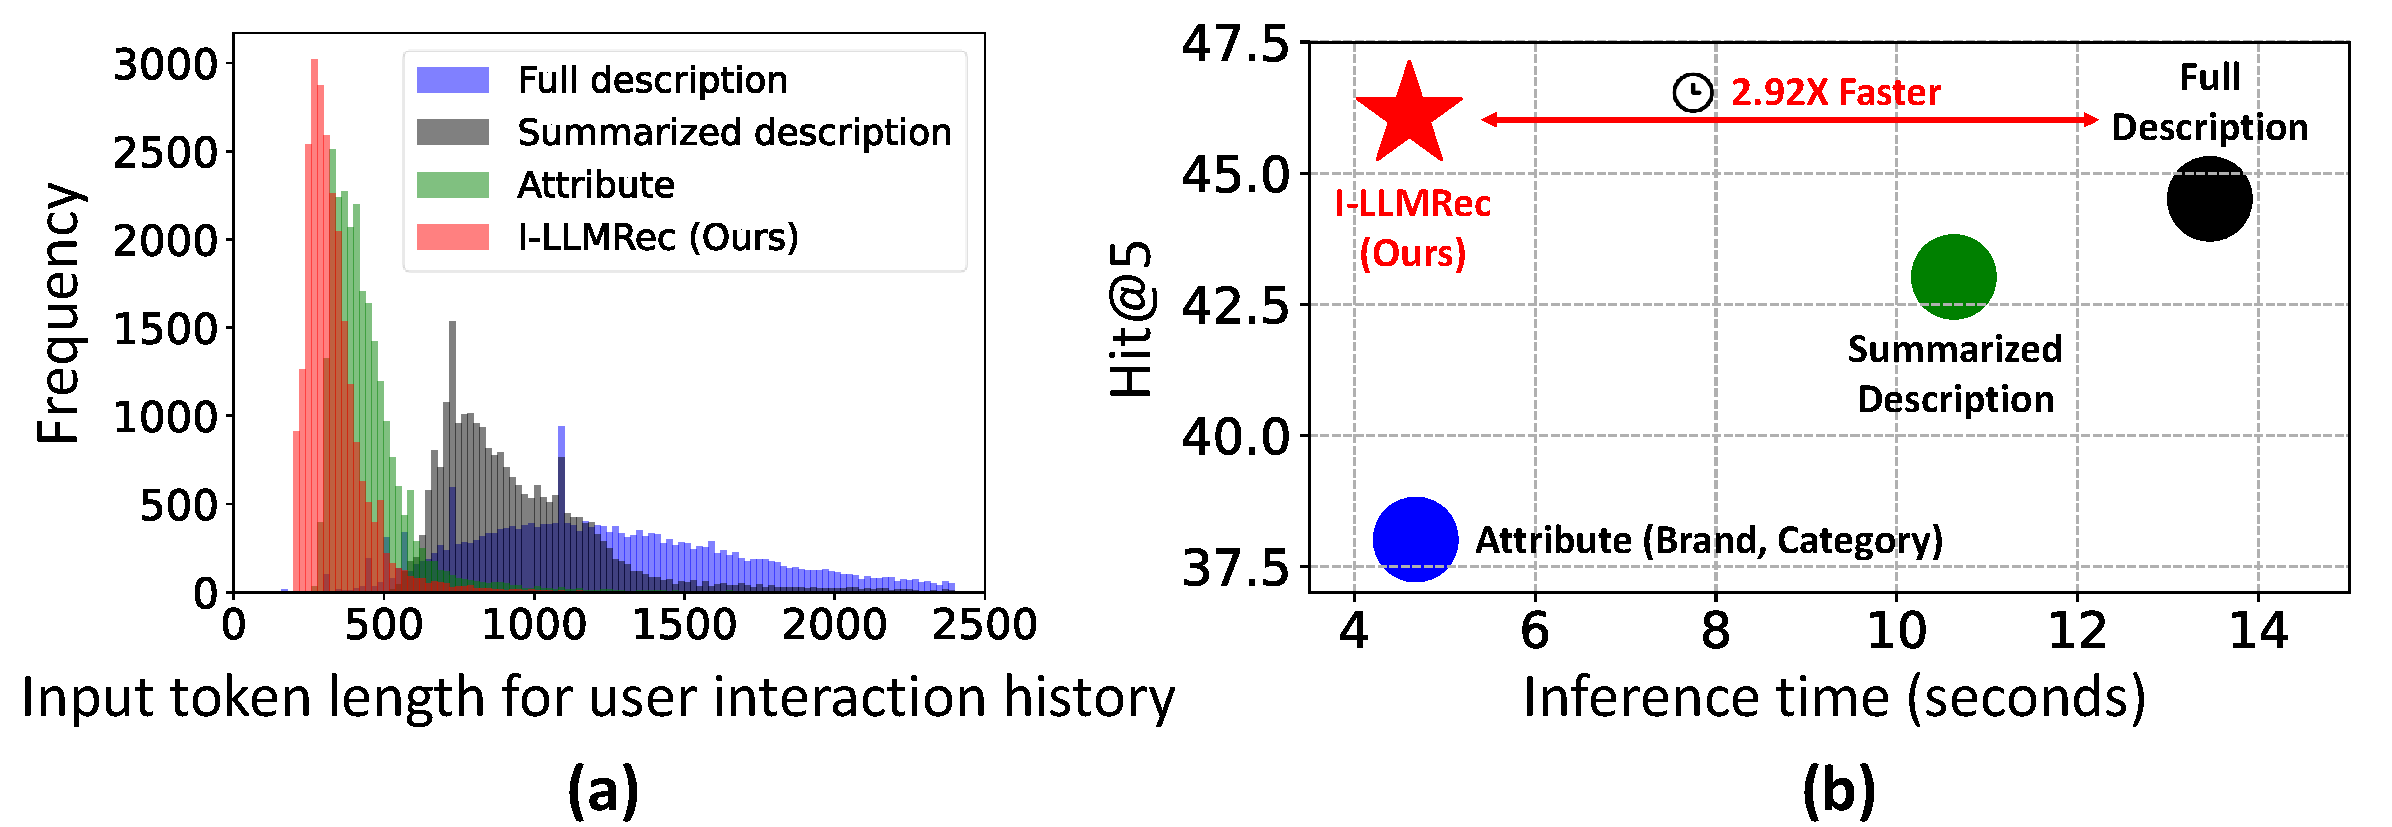
\includegraphics[width=0.99\linewidth]{Figure/Intro_Figure.pdf}
  \vspace{-1ex}
  \caption{(a) Histogram of the input token length required to represent a user's item interaction history across different item expression approaches. (b) Recommendation performance (Hit@5) and Inference Time (seconds/100 users) for different item representation approaches. We use the Amazon Sports dataset for analysis.}
  \label{fig:intro}
    \vspace{-1.0ex}
\end{figure}


The key to LLM-based recommender systems lies in effectively representing items in natural language to capture user preferences based on LLM's comprehensive understanding of user interaction history. In this regard, existing studies that represent items in natural language can be categorized into the following two main approaches:
\textbf{1) Attribute-Based Representation} approach is to combine simple attributes such as brand and category with the item title to represent the item \cite{bao2023tallrec,li2023text,tan2024idgenrec,lin2024bridging}. For example, TALLRec \cite{bao2023tallrec} represents items with their title for user preference modeling, while RECFORMER \cite{li2023text} enhances user preference understanding by adding brand and category attributes with attribute type-specific tokens in the prompt. Similarly, TransRec \cite{lin2024bridging} incorporates attribute information alongside the title in the prompt to facilitate a multifaceted understanding of items.
\textbf{2) Description-Based Representation} approach is to use detailed item descriptions to preserve rich textual item semantics so that the LLM could capture user preference in a more fine-grained manner. For example, TRSR \cite{zheng2024harnessing} summarizes full descriptions using a large-scale LLM and provides them to a small-scale  LLM for recommendation, thereby overcoming the limited item semantics provided by attributes only and addressing the input length constraints of LLMs (e.g., 1,024 tokens for GPT-2 \cite{radford2019language}).

However, \textit{we argue that the two aforementioned approaches inherently face a trade-off between efficiency and effectiveness when representing items}. Specifically, the
Attribute-Based Representation approach is efficient since it requires fewer tokens to add item attributes than to add the entire item descriptions, which shortens the input length for the LLM\footnote{Since LLMs are built on transformers, their computational complexity grows quadratically as the input token length increases.}. However, it sacrifices the effectiveness of understanding user preferences due to the limited item semantics that can be contained in relatively short attributes. On the other hand, the 
Description-Based Representation approach is less efficient due to the longer input length required for detailed item descriptions, whereas the effectiveness of understanding user preferences is improved by utilizing richer textual semantics of items. 
% Regarding an actual input length required to represent a user interaction history, we show it in Figure~\ref{fig:intro}(a), indicating that Description-based approach (i.e., Summarized description\footnote{To summarize the full description, we adopt an approach similar to TRSR \cite{zheng2024harnessing} and use similar prompt. For more details, please refer to Appendix.} and Full description) demands much longer input lengths than Attribute-based Representation approach (i.e., Attribute), resulting in the increased computational complexity.
In fact, as shown in Figure~\ref{fig:intro}(a), the input length required for LLMs to represent a user's item interaction history significantly varies depending on how the item is represented. That is, the Description-Based Representation approach (i.e., Summarized description\footnote{To summarize the full description, we adopt an approach similar to TRSR \cite{zheng2024harnessing} and use a similar prompt. For more details, please refer to Appendix~\ref{app_sec:prompt4summarization}.} and Full description) demands much longer input token lengths than the Attribute-Based Representation approach (i.e., Attribute), resulting in the increased computational complexity.

% To gain a deeper understanding of this trade-off, we go beyond merely comparing the input token length, and compare the computational complexity of different item representation approaches in terms of training and inference (Figure~\ref{fig:intro}(b)). 
To better understand this trade-off, in Figure 1(b), we extend our analysis beyond a simple comparison of input token length and examine the computational complexity of different item representation approaches (i.e., efficiency) along with their recommendation performance (i.e., effectiveness).
Note that we use the same LLM backbone (i.e., Sheared LLaMA-2.7B \cite{xia2023sheared}) and adopt the same recommendation protocol for fair comparisons (See Appendix~\ref{app_sec:rec_protocol} regarding the details of recommendation protocol).
% we conduct experiments under the same recommendation protocol and using the 
% same LLM (i.e., Sheared LLaMA-2.7B \cite{xia2023sheared}) as the recommendation backbone, while varying across different item representation approaches.
% Beyond comparing the input length for different item representation approaches, to clearly understand this trade-off, we conduct experiments using the same recommendation protocol and the 
% same LLM (i.e., Sheared LLaMA-2.7B \cite{xia2023sheared}) as the recommendation backbone, while varying only the item representation approach.
% Specifically, we compare the inference time and the recommendation performance, each of which is responsible for efficiency and effectiveness, respectively. 
% As shown in Figure~\ref{fig:intro}(b), 
We observe that the Attribute-based Representation approach (blue circle) achieves the inference time more than 2.5 times faster than the Description-based Representation approach (green and black). However, this comes at the expense of a performance reduction of over 13\% due to the lack of rich item semantics contained in attributes compared with descriptions.
% loss of item's richer semantic information provided by the descriptions in comparison with attributes.
Furthermore, summarizing full descriptions reduces inference time but compromises performance due to the information loss during the summarization process. 
In conclusion, the trade-off can be summarized as: \textit{richer (i.e., longer) item representation provided to the LLM improves effectiveness but decreases efficiency}. However, this trade-off is unavoidable by nature if items are to be represented with natural language.
% due to demonstrates shorter inference times but shows lower performance due to limited item's information. On the other hand, the Description-based Representation (green and black circles) approach requires longer inference times while achieving  higher performance by leveraging richer item representation. 




\begin{figure}[t]
  \centering
  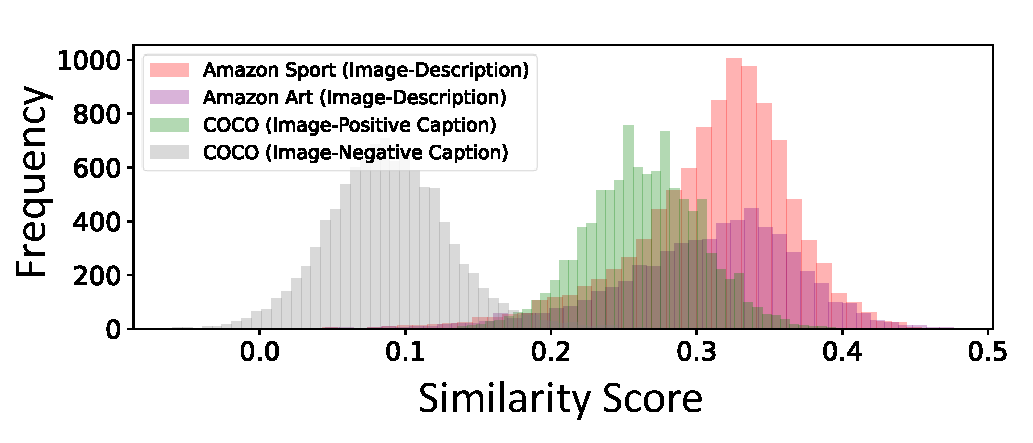
\includegraphics[width=0.95\linewidth]{Figure/Intro_Figure2.pdf}
  \vspace{-1ex}
  \caption{Cosine similarity between item image-description pairs in Amazon Sport and Art datasets and image-caption pairs in the COCO dataset using CLIP \cite{radford2021learning}.}
  % For the item set, we use the Amazon Sport dataset.
  \label{fig:intro2}
  \vspace{-1ex}
\end{figure}



In this paper, we focus on addressing this trade-off based on our interesting observation that there is a significant information overlap between images and descriptions associated with items. Specifically, when we measure the similarity between item image-description pairs in a real-world e-commerce dataset (i.e., Amazon Sport and Art \cite{ni2019justifying}) using a vision-language model (i.e., CLIP \cite{radford2021learning}) in which image and language spaces are jointly embedded, we found that the similarity is surprisingly high. Specifically, Figure~\ref{fig:intro2} shows that the average similarity for the Amazon Sport and Art datasets is around 0.31. To better understand this similarity level, we conducted the same experiment with the COCO caption dataset \cite{lin2014microsoft}, a well-curated image-caption pair dataset widely used in vision-language research. Specifically, we measured similarities for both positive (i.e., image-caption) and negative (i.e., image-randomly sampled unrelated caption) pairs.
% \footnote{For the negative caption of an image, we randomly sampled a caption from COCO dataset.}. 
Given that the negative pairs have an average similarity of only 0.07, the positive pairs' average similarity of around 0.26 can be considered an indicator of high similarity. 
Furthermore, the similarity value of 0.31 between item image-description pairs, which is even higher, highlights a significant information overlap between images and their associated descriptions\footnote{Such an observation was consistently observed across other real-world datasets as well as another CLIP variant model (See Appendix~\ref{app_sec:overlap_other_dataset}).}.
% This demonstrates that the the similarity value of 0.31 between item image-description pairs is indeed very high, demonstrating that there is a significant information overlap between images and descriptions associated with items\footnote{Such an observation was consistently observed across other real-world datasets as well as another vision-language model (See Appendix~\ref{app_sec:overlap_other_dataset}).}.
% is indeed high in that the average similarity even exceeds that of the COCO positive pairs. 


 % We observed that compared to an average similarity of 0.07 within image-negative caption pairs, the image-positive caption pairs exhibit a significantly higher similarity of an average similarity of 0.26 while highly exceeding this similarity, demonstrating that the information overlap between images and descriptions associated with items is indeed high. Such an observation was consistently observed across other real-world datasets as well (See Appendix~\ref{app_sec:overlap_other_dataset}).

% To validate the level of similarity, we conduct the same experiment with the COCO caption dataset \cite{lin2014microsoft}, which is a well-curated image-caption pair dataset widely used in vision-language research.
% We observe that the average similarity is around 0.28 for the COCO dataset,   
% demonstrating that the information overlap between images and descriptions associated with items is indeed high. Such an observation was consistently observed across other real-world datasets as well (See Appendix~\ref{app_sec:overlap_other_dataset}).

% Figure~\ref{fig:intro2}(b), given that the average cosine similarity for COCO pairs is 0.24, the 0.55 average cosine similarity observed for item pairs is significantly higher, further confirming this overlap. Such an observation was consistently observed across other real-world datasets as well (See Appendix~\ref{app_sec:overlap_other_dataset}).}
% an average cosine similarity of 0.55 for item pairs, which is considerably higher than the 0.24 observed for COCO pairs, further confirming this overlap. Such an observation was consistently observed across other real-world datasets as well (See Appendix~\ref{app_sec:overlap_other_dataset}).
% we discovered a breakthrough solution to addressing the trade-off by identifying 
% Specifically, 
% Specifically, we employed SigLIP \cite{zhai2023sigmoid}, a variant of CLIP \cite{radford2021learning} with sigmoid loss function, and analyzed the sigmoid-based similarity between item image-description\footnote{Summarized descriptions are used instead of full descriptions due to the limited input size of the text encoder in the vision-language model.} pairs. As shown in Figure~\ref{fig:intro2}(a), most items exhibit a similarity score close to 1 in a real-world dataset (i.e., Amazon Sport \cite{ni2019justifying}), demonstrating a significant overlap between images and descriptions associated with items. 
% To further explore this overlap, we compute the cosine similarity between the item image-description pairs using the commonly used CLIP \cite{radford2021learning} encoders, and compare it with the image-caption pairs in the COCO dataset \cite{lin2014microsoft}, which is a widely used dataset in vision-language model research.
% % \textcolor{red}{To further explore this overlap, we use CLIP \cite{radford2021learning} commonly used and compute the cosine similarity of COCO image-caption pairs for relative comparison while computing that of the item image-description pairs.}
% As shown in Figure~\ref{fig:intro2}(b), we observed an average cosine similarity of 0.55 for item pairs, which is considerably higher than the 0.24 observed for COCO pairs, further confirming this overlap. Such an observation was consistently observed across other real-world datasets as well (See Appendix~\ref{app_sec:overlap_other_dataset}).

% Building on this observation, we propose a novel method, \textbf{I}mage is all you need for \textbf{LLM}-based \textbf{Rec}ommender system (\proposed{}), which kills two birds (i.e., efficiency and effectiveness) with one stone (i.e., image) as an alternative to lengthy descriptions for item expression, thereby reducing token usage while preserving rich item semantics of the descriptions
Building on this observation, we propose a novel method, \textbf{I}mage is all you need for \textbf{LLM}-based \textbf{Rec}ommender system (\proposed{}), which addresses both efficiency and effectiveness of existing LLM-based recommender systems by leveraging images as an alternative to lengthy textual descriptions for the item expression, aiming at reducing token usage while preserving the rich semantic information of item descriptions\footnote{Some text-specific information that is missing in an image may be lost, but we find that in Section~\ref{sec:performance}, this information has surprisingly little impact on recommendations.}. 
% The core idea is for the LLM to deeply understand items interacted by users through images rather than descriptions. 
% allowing it to effectively capture user preferences. 
The main technical challenge lies in the misalignment between the item image space and the language space.
% However, there exists a challenge in that the item image space and the language space are not aligned.
To this end, we adopt a learnable adaptor for visual features followed by
% that makes image features compatible with the language space and 
% the Recommender Image-LLM Alignment (Rec-ILA) mode 
a technique to bridge the gap between the two spaces (i.e., Image-LLM Alignment mode (ILA)), which facilitates the training of the adaptor with carefully crafted prompts tailored to the recommendation context. 
This ensures the LLM to capture rich item semantics through images with only a few tokens, thereby effectively and efficiently capturing user preferences.

% Furthermore, they rely on computationally intensive beam search for recommending multiple items
% However, these approaches suffer from the following limitations: 
% (1) they rely on computationally intensive beam search for recommending multiple items, (2) they cannot guarantee that the recommended items exist within the item corpus (i.e., lack of item grounding), and (3) they require an oversized LLM as expanding the item pool necessitates extending the OOV, which hinders scalability\footnote{Limitations (1) and (2) are related to the next title prediction approach, while limitation (3) is associated with the item token prediction approach.}

% Moreover, beyond merely using images to enhance item semantics for user preference understanding, we propose the Image-based REtrieval (IRE) mode, a retrieval-based recommendation approach that leverages images to directly retrieve relevant items from the item pool. Existing studies on LLM-based recommender systems typically recommend items by predicting the next item title \cite{kim2024large,lin2024bridging,tan2024idgenrec} or item tokens allocated as out-of-vocabulary (OOV) \cite{wei2024towards,li2023text,geng2023vip5,zhu2024collaborative}. However, these approaches suffer from the following limitations: 
% (1) they rely on computationally intensive beam search for recommending multiple items, (2) they cannot guarantee that the recommended items exist within the item corpus (i.e., lack of item grounding), and (3) they require an oversized LLM as expanding the item pool necessitates extending the OOV, which hinders scalability\footnote{Limitations (1) and (2) are related to the next title prediction approach, while limitation (3) is associated with the item token prediction approach.}. By introducing image-based retrieval for recommendations, we address these limitations, providing a more efficient and reliable recommender systems.




Through extensive experiments on various real-world datasets, we demonstrate that our proposed method using images instead of item descriptions is superior in both effectiveness and efficiency. Specifically, \proposed{} improves inference speed by approximately 2.93 times compared to the Description-based Representation approach, while achieving a 22\% performance improvement over the Attribute-based Representation approach (Figure 1(b)). As a further appeal, \proposed{} facilitates robust recommendations by mitigating sensitivity to noise associated with item descriptions as it relies on images. Our main contributions can be summarized as follows:


    % \item We propose a new image-based retrieval recommendation approach to provide more efficient and reliable recommendation.
\begin{itemize}[leftmargin=5mm]
    \item {We identify a trade-off between efficiency and effectiveness when expressing items in natural language.}
    \item  {Based on the observation that there is a significant overlap between item image-description pairs, we propose a novel method, called \proposed{}, which utilizes images instead of textual descriptions to efficiently and effectively capture user preferences.}
    \item {Our extensive experiments demonstrate that \proposed{} outperforms the various natural language-based representation approaches in both effectiveness and efficiency.}
\end{itemize}

% Contributions
% We identify the trade-off between effectiveness and efficiency in existing LLM-based recommendation methods that rely on textual (description) representations of items.
% We discover a novel insight that item descriptions and image information exhibit a high degree of redundancy. Based on this, we propose a methodology that leverages image features to alleviate the trade-off between effectiveness and efficiency.
% Through extensive experiments, we validate that the proposed approach outperforms existing methods in terms of both effectiveness and efficiency.





\section{Preliminary}
In this section, we first introduce the task formulation and then examine the complexity of different item expression approaches.

\smallskip
% \subsubsection{\textbf{Task Formulation}}
\noindent\textbf{Task Formulation. }
Throughout this paper, we mainly focus on sequential recommendation, as it closely aligns with real-world scenarios \cite{tian2022multi,xie2022decoupled}.
Let $\mathcal{U}$ and $\mathcal{I}$ denote the set of users and items, respectively. A user $u\in \mathcal{U}$ has the historical item interaction sequence denoted as $\mathcal{S}_u$=[$i_1, i_2, ..., i_k, ..., i_{|\mathcal{S}_{u}|}$], where $i_k$ denotes the $k$-th interacted item and $|\mathcal{S}_u|$ is the number of items in the interaction sequence. The goal of this task is, for each user $u$, to predict the next item $i_{|\mathcal{S}_u|+1}$ to be consumed by the user based on the user interaction history $\mathcal{S}_u$.

% to design a score function for the next item, $\mathcal{T}: i \rightarrow  \mathbb{R}$ $\forall i \in \mathcal{I}$, based on the user interaction history $\mathcal{S}_u$, and then recommend the next item $i_{|\mathcal{S}_u|+1}$ with high scores. 

\smallskip
% \subsubsection{\textbf{Expression of Item Semantics}}
\noindent\textbf{Representing Item Semantics. }
With the advancement of LLMs for recommender systems, there is a growing need to help them understand the semantics of items to capture user preferences. In this regard, we categorize the multiple types of information to recommend an item $i$'s semantics into [$\mathbf{I}_i$, $\mathbf{D}_i$, $\mathbf{A}_i$], where $\mathbf{I}_i$, $\mathbf{D}_i$, and $\mathbf{A}_i$ are an item image, textual description\footnote{To avoid confusion, we will henceforth refer to the description as summarized description instead of full description unless stated otherwise.}, and attribute (e.g., brand and category), respectively. 
% In the real world, the item $i$ contains multiple type of information, such as ite 
% Extending the conventional sequential recommendation task, we follow the  assumption of the previous studies \cite{wei2024towards,geng2023vip5,zheng2024harnessing} that each item $i \in \mathcal{I}$ is enriched with multiple types of information formed as \{$\mathbf{I}_i$, $\mathbf{D}_i$, $\mathbf{A}_i$\}, where $\mathbf{I}_i$, $\mathbf{D}_i$, and $\mathbf{A}_i$ is an image, detailed description, and attribute (e.g., brand and category) for an item $i$, respectively.Nevertheless,
%  we further relax this assumption of complete type of information, and present experiments in Section~\ref{exp:missing} for cases where each type of information is missing.

\smallskip
% \subsubsection{\textbf{Comparison of complexity.}}
\noindent\textbf{Comparison of complexity.}
Let $f(\cdot)$ denote the transformation function for the LLM to convert the representation of item semantics into input tokens, and let $|f(\cdot)|$ denote the number of input tokens. Specifically, for $\mathbf{D}_i$ and $\mathbf{A}_i$ that are in natural language, $f$ refers to tokenizing the natural language and converting them into the word embeddings. Meanwhile, for an image $\mathbf{I}_i$, $f$ involves extracting the visual features using a pretrained vision encoder (e.g., CLIP-ViT \cite{radford2021learning}), followed by an adaptor to resize their feature dimensions for compatibility with the LLM \cite{liu2024visual,li2023blip}. The complexity of LLM operations for each representation is $O((|f(\mathbf{I}_i)| |\mathcal{S}_u|)^2d)$, $O((|f(\mathbf{D}_i)| |\mathcal{S}_u|)^2d)$, and $O((|f(\mathbf{A}_i)| |\mathcal{S}_u|)^2d)$, where $|f(\mathbf{D}_i)| >> |f(\mathbf{A}_i)|$. This is derived based on the complexity of Transformer, i.e., $O(n^2d)$, where $n$ is the input token length and $d$ is the feature dimension of the LLM. It reveals that the complexity of the description-based approach is not merely being incurred with a single item; rather, it increases with the user sequence length $|\mathcal{S}_u|$, and its complexity even grows quadratically, making this approach impractical.
% On the other hand, the complexity of the attribute-based approach is 
% tolerates to add the attributes with lower complexity. 
% In this vein, it reminds us of the importance of reducing the complexity required to express even a single item. 
% In this regard, we argue that it is important to reduce the complexity required to express even a single item
Therefore, in this work, we propose to lower the complexity of expressing an item by leveraging its associated image using only a single token (i.e., $|f(\mathbf{D}_i)| \gg |f(\mathbf{A}_i)| > |f(\mathbf{I}_i)|=1$ )\footnote{In average, $|f(\mathbf{D}_i)|$ and $|f(\mathbf{A}_i)|$ are approximately 160 and 10 tokens, respectively.} while preserving the rich semantics of the item description. This is based on our observation that there is a significant information overlap between the item image-description pairs (Figure~\ref{fig:intro2}).

% description approach is intolerant since $f(\mathbf{D}_i)$ per item is too lengthy, and its complexity grows quadratically as the user sequence length $|\mathcal{S}_u|$ increases, which intensifies the complexity for LLMs.

% \vspace{-1ex}
\section{Proposed Method: \proposed{}}
In this section, we provide a detailed explanation of \proposed{}.
After introducing the initial recommendation-related task prompt, we begin by encoding the images of items consumed by users, and mapping them to an LLM through a learnable adaptor (Section~\ref{sec:map}).
However, since these mapped visual features are not inherently aligned with the language space, we propose the Image-LLM Alignment (ILA) module that trains the adaptor with carefully crafted prompts tailored for the recommendation context, resulting in effectively bridging the alignment gap (Section~\ref{sec:alignment}). Meanwhile, we propose the Image-based REtrieval (IRE) module, a training approach that enables the LLM to directly perform recommendations from the item corpus based on the visual features (Section~\ref{sec:retrieval}). Finally, we describe the overall training objectives and inference for recommendation (Section~\ref{sec:training} and \ref{sec:inference}). The overall framework of \proposed{} is shown in Figure~\ref{fig:main}.

% \vspace{-1ex}
\subsection{Mapping Item Images to LLM}
\label{sec:map}
Recall that, as shown in Figure~\ref{fig:intro2}, the item image contains rich item semantics of the lengthy description. Therefore, in this section, our goal is to map items consumed by users to an LLM using only a few tokens, allowing us to capture user preference efficiently and effectively. 
%\mathcal{S}_u^{\mathbf{I}}, \mathcal{\hat{S}}_u^{\mathbf{I}}=
Specifically, 
given the interaction history of user $u$, i.e., $[i_i, i_2, ..., i_{|\mathcal{S}_u|-1}]$, and a target item $i_{|\mathcal{S}_u|}$, we convert the interaction history into a sequence of item images $[\mathbf{I}_{i_1}, \mathbf{I}_{i_2}, ... , \mathbf{I}_{i_{|\mathcal{S}_u|-1}}] \in \mathbb{R}^{(|\mathcal{S}_u|-1) \times H \times W \times 3}$, where $H$ and $W$ are the image height and width, respectively. Then, we adopt a pretrained visual encoder $V$ of a vision-language model to extract the visual features of each item, defined as $v_i = V(\mathbf{I}_i) \in \mathbb{R}^{d_v}$. This process makes the sequence of visual features $[v_{i_1}, v_{i_2}, ..., v_{i_{|\mathcal{S}_u|-1}}] \in \mathbb{R}^{(|\mathcal{S}_u|-1)\times d_v}$, where $d_v$ is the dimension of the visual feature. 

\subsubsection{\textbf{Adaptor network for visual features.}} However, since the visual feature dimension $d_v$ is different from that of the LLM feature $d$, and their spaces are inherently misaligned, we introduce an adaptor network $M:\mathbb{R}^{d_v} \rightarrow \mathbb{R}^{d}$ to make visual features compatible with the LLM's feature dimension, allowing $v_i$ to be interactive with word embeddings within the LLM's input layer. 
More precisely, we process each item's visual feature \( v_i \) through the adaptor \( M \), transforming it into a sequence of visual features that match the dimensionality of the LLM. Formally, we the sequence of mapped visual features is defined as:
% More precisely, we feed-forward each item's visual feature $v_i$ through the adaptor $M$, making the sequence of visual features whose dimension is same with the LLM, formally defining the user interaction history as:
%\mathcal{\hat{S}}_u^{\mathbf{I}}
\begin{equation}
    \mathcal{\bar{S}}_u^{\mathbf{I}}=[\bar{v}_{i_1}, \bar{v}_{i_2}, ..., \bar{v}_{i_{|\mathcal{S}_u|-1}}], \bar{v}_i=M(v_i) \in \mathbb{R}^d.
\end{equation}
% \noindent where $\mathcal{\bar{S}}_u^{\mathbf{I}}$ is the sequence of mapped visual features for the LLM.



\begin{figure*}[t]
  \centering
  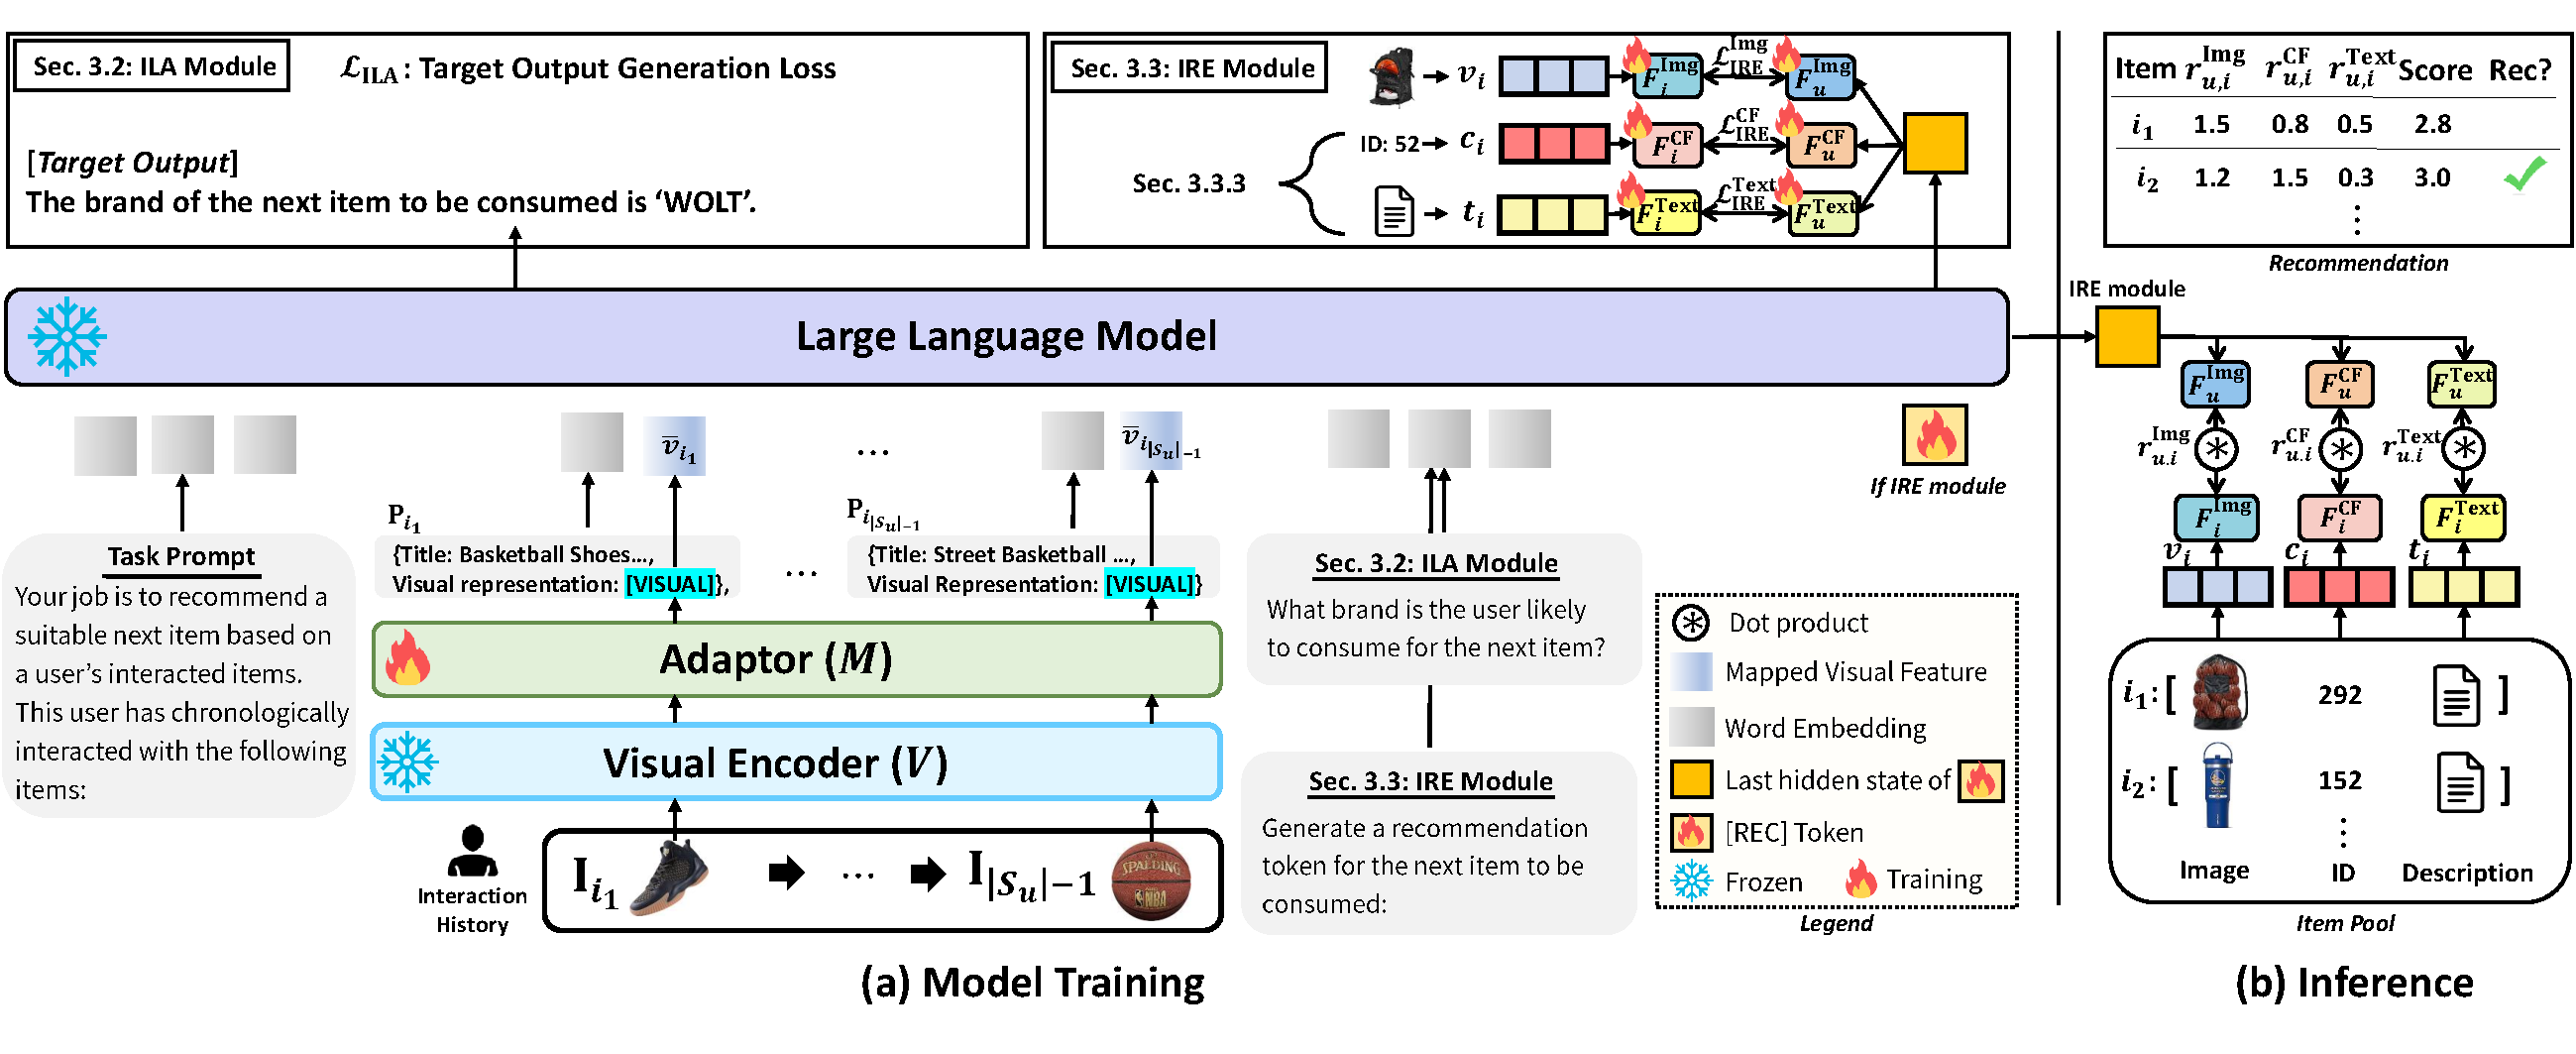
\includegraphics[width=0.92\linewidth]{Figure/main_figure.pdf}
  \vspace{-1ex}
  \caption{Overall framework of \proposed{}. User-interacted item images are mapped into the LLM through an adaptor, which bridges the image and language spaces. To ensure alignment between two spaces, the adaptor is optimized via the ILA module. Furthermore, the recommendation process is formulated as a retrieval task via the IRE module.
  }
  \vspace{-1ex}
  \label{fig:main}
\end{figure*}

% \vspace{-2ex}
\subsubsection{\textbf{Designing a prompt to represent a user's item interaction history.}} 
To represent a user's item interaction history with visual features, we carefully design a prompt, enabling the LLM to comprehensively understand the item semantics.
% Based on the $\mathcal{\bar{S}}_u^{\mathbf{I}}$ containing the rich item semantics, we design the prompt to express the user interaction with visual features. 
Specifically, for each item $i$ in a user's item interaction history, we represent it in the prompt as follows:
\vspace{-0.1ex}
\begin{equation}
    \mathbf{P}_i=\left\{ \textrm{Title}: \textsf{ITEM\_TITLE}, \textrm{Visual}\; \textrm{Representation}: \left[ \textsf{VISUAL} \right] \right\}
    \label{eqn:2}
\end{equation}
where $\mathbf{P}_i$ is the representation of item $i$ in the prompt, $\textsf{ITEM\_TITLE}$ is the title of the item $i$, and $\left[ \textsf{VISUAL} \right]$ is the placeholder of item $i$'s visual feature $\bar{v}_i$. 
More precisely, before being forwarded to the LLM's transformer layer, $\left[ \textsf{VISUAL} \right]$ is replaced with $\bar{v}_i$, while the natural language in $\mathbf{P}_i$ is converted into word embeddings. 
Note that following prior studies \cite{bao2023tallrec,li2023text}, we use the item title instead of the item's numerical ID.
% used in traditional collaborative filtering models, expressing the unique item in natural language. 
By enumerating $\mathbf{P}_i$ over the item interaction history of user $u$ (i.e., $[\mathbf{P}_{i_1}, \mathbf{P}_{i_2}, ..., \mathbf{P}_{i_{|\mathcal{S}_u|-1}}]$), we represent the user interaction based on item images where each image is expressed using a single token, allowing the LLM to efficiently and effectively capture the user preference.

% To train the adaptor $M$ effectively, we propose the instruction mode and recommendation mode, each of which is designed to create the instruction prompt tailored to recommendation context, and utilizes retrieval-based recommendation approach by optimizing the recommendation loss of negative log-likelihood. 

\vspace{-1.3ex}
\subsection{Image-LLM Alignment (ILA) Module}
\label{sec:alignment}
To make the LLM effectively capture user preferences from item images, it is crucial to align visual features with the language space in a meaningful way, requiring adequate supervision of the adaptor network $M$. 
% Without this, the LLM may struggle to interpret item semantics from images, limiting its effectiveness.
To achieve this, we optimize the adaptor network $M$ by predicting the next item properties based on the user interaction within a structured prompt. This approach ensures that the LLM learns to associate visual features with relevant textual information, thereby improving its ability to understand user preferences in the context of recommendation.
% is well-aligned with the sequential recommendation task for the next item prediction, ensuring that the LLM learns to associate visual features with relevant textual information, thereby improving its ability to understand user preferences in the context of recommendation.

% to be interacted based on the user interaction history with image features, resulting in effectively aligning the user-interacted item features to the language space.

Specifically, we craft a prompt in an $\textit{"input"}$-$\textit{"target output"}$ format. Here, the $\textit{input}$ consists of the user interaction prompt, followed by a question regarding the next item (e.g., \textit{What brand is this user likely to consume for the next item?}). The \textit{target output} corresponds to the answer to that question (e.g., \textit{The brand likely to be consumed is `WOLT'}). To guide the LLM in considering various properties of the next item, we incorporate multiple properties of the next item, including brand, category, title, and description. For each property, we design five different question templates (refer to Appendix~\ref{app_sec:question} for complete templates). During each training step, we randomly select one of 20 possible question templates (4 properties × 5 templates) and train $M$ to generate the corresponding output. The training objective is formulated as follows:
\begin{equation}
    \mathcal{L}_{\text{ILA}}=\underset{M}{\textrm{max}}\sum_{k=1}^{|y|}log(P_{\theta,M}(y_k|x,y_{<k}))
    \label{eqn:ila}
\end{equation}
where $\theta$ is the parameter of the LLM that is frozen, $y$ is the \textit{target output}, $y_k$ is the $k$-th token of $y$, and $x$ is the \textit{input}.

\smallskip
\subsubsection{\textbf{Discussion regarding LLM fine-tuning}}
% In the LLM-based recommendation studies, fine-tuning has been a necessary but resource-intensive process for capturing user preferences. On the other hand, \proposed{} offers a key advantage by eliminating the need for fine-tuning, instead leveraging the LLM’s intrinsic knowledge to generate recommendations. While fine-tuning could potentially enhance performance (see Appendix for details), we choose to keep the LLM frozen to maintain its inherent knowledge and optimize training efficiency. Ultimately, the ability to train the model without fine-tuning the LLM further emphasizes efficiency, which remains one of our primary goals.
A further benefit of \proposed{} is that LLM fine-tuning is not mandatory, unlike the existing LLM-based recommender systems \cite{lin2024bridging,bao2023tallrec,tan2024idgenrec,zheng2024harnessing,liu2024once} that generally rely on costly fine-tuning of the LLM. Instead, we harness the LLM's intrinsic parametric knowledge to understand the user preferences. Even though \proposed{} could be potentially improved by fine-tuning the LLM (See Appendix~\ref{app_sec:fine_tune}), we opt to keep the LLM frozen to preserve the LLM's intrinsic knowledge and improve the training efficiency.
% , further emphasizing the advantage of efficiency.  

% Unlike the existing studies for LLM-based recommender systems, we keep the LLM frozen. In other words, while existing studies tend to fine-tune the LLM to learn user preferences, we just harness its semantic reasoning to infer them, preserving the LLM's intrinsic knowledge.

% \vspace{-1.5ex}
\subsection{Image-based REtrieval (IRE) Module}
\label{sec:retrieval}
We found that existing studies on LLM-based recommender systems often face challenges in providing \textit{reliable} and \textit{efficient} recommendations. This is because they typically recommend items by predicting the next item title \cite{kim2024large,lin2024bridging,tan2024idgenrec} or item tokens allocated as out-of-vocabulary \cite{wei2024towards,li2023text,zhu2024collaborative}. Regarding \textit{reliable} recommendation, the title prediction approach cannot guarantee that the recommended items exist within the item corpus (i.e., lack of item grounding), which sometimes may lead to recommending non-existent items.
% That is, since the LLM does not have complete knowledge of all items, it may generate recommendations of non-existent items.
% as the LLM does not have complete knowledge of all items, likely to recommend non-existent items. 
Regarding \textit{efficient} recommendation, title prediction relies on computationally intensive beam search to recommend multiple items, while the item token prediction approach requires an oversized LLM, as expanding the item pool necessitates extending the LLM vocabulary set, which hinders scalability. To overcome these challenges, we propose the Image-based REtrieval (IRE) module, which formulates the recommendation task as a retrieval task by leveraging the images to directly retrieve relevant items from the item pool.
% As discussed in Section~\ref{sec:intro}, prior studies often struggle to provide \textcolor{red}{reliable (CY: reliable 이야기는 없던것 같은데, 다시한번 앞에서 이야기한것과 잘 매칭이 되게 서술하고있는지 확인해주세요.)} and efficient recommendations for the next item.
% due to either prediction of the item title or item token allocated by OOV.
% To overcome these, we formulate the recommendation process as a retrieval task by leveraging item visual features.
% beyond the utilization them for user preference understanding. 
% Last: As we perform recommendations by directly retrieving the relevant items, we can guarantee the item existence in the item corpus and do not have to extend the item tokens within the LLM, making the reliable and efficient recommendation. 
In the following, we describe how to obtain an LLM-guided user representation for retrieval, and define a training objective that retrieves relevant items using the visual features.


% To transform the recommendation process into a retrieval task, we modify the input prompt structure and introduce a special token that aggregates 
% to transform the recommendation process into a retrieval task,
\subsubsection{\textbf{LLM-guided user representation}} 
To obtain the LLM-guided user representation containing user preference, for each user $u$, we append an instruction prompt, i.e., \textit{Generate a recommendation token for the next item to be consumed}, after the user interaction prompt $[\mathbf{P}_{i_1}, \mathbf{P}_{i_2}, ..., \mathbf{P}_{i_{|\mathcal{S}_u|-1}}]$. This instruction prompt helps generate a recommendation token, guiding the model towards item retrieval-based recommendations instead of item title generation-based recommendation. At the end of this prompt, we append a learnable token \rectoken{} that aggregates a user's item interaction history and instruction-related information, leveraging the LLM's contextual reasoning capabilities. Specifically, we utilize the last hidden state associated with the \rectoken{} token (i.e., $h$(\rectoken{})) to obtain the aggregated information of user preference for retrieval.  
\subsubsection{\textbf{Training objective for retrieving relevant items}} Given that $h$(\rectoken{}) represents the user's preference contained in the interaction history of user $u$, i.e., [$i_1, i_2,...,i_{|\mathcal{S}_u|-1}$], we formulate the task of retrieving the target item $i_{|\mathcal{S}_u|}$ based on a scoring function $\mathcal{T}$, unlike previous studies relying on a generative task (i.e., item title generation). To this end, we use the visual feature of items as the item representations and compute the affinity score between those and $h$(\rectoken{}).
% , defining the $\mathcal{T}$.
However, as $h$(\rectoken{}) and the visual features lie in the different spaces, we employ projectors for each, ensuring that they are mapped into a shared recommendation space. We denote the projectors and their outputs as follows:
\begin{equation}
    o_u^{\textsf{Img}}=F^{\textsf{Img}}_u(h(\left[ \texttt{REC} \right])), o_i^{\textsf{Img}}=F^{\textsf{Img}}_i(v_{i_{|\mathcal{S}_u|}})
    \label{eqn:4}
\end{equation}
where $F^{\textsf{Img}}_u:\mathbb{R}^d \rightarrow \mathbb{R}^{d_{s}}$, $F^{\textsf{Img}}_i:\mathbb{R}^{d_{v}} \rightarrow \mathbb{R}^{d_{s}}$ are the projectors, and $d_s$ is the feature dimension of shared recommendation space. $o_u^{\textsf{Img}}$ and $o_i^{\textsf{Img}}$ denote the projected representations of user $u$ and item $i$ in terms of visual features, respectively. 
To optimize the retrieval task,
we use the binary cross-entropy loss
as the training objective:
\begin{equation}
\begin{split}
    \mathcal{L}_{\text{IRE}}^{\textsf{Img}} &= -\sum_{u \in \mathcal{U}}\left[ log(\sigma(r_{u,i}^{\textsf{Img}}))+log(1-\sigma(r_{u,i^-}^{\textsf{Img}})) \right] 
    % \mathcal{T}=o_{u}^v \circledast o_{i}^v
\label{eqn:5}
\end{split}
\end{equation}
where $r_{u,i}^{\textsf{Img}} =\mathcal{T}(o_u^{\textsf{Img}},o_i^{\textsf{Img}}) = o_u^{\textsf{Img}} \circledast o_i^{\textsf{Img}} \in \mathbb{R}$ is the affinity score between $o_u^{\textsf{Img}}$ and $o_i^{\textsf{Img}}$, with $\circledast$ denoting the dot product, and $i^-$ is a randomly selected negative item. It is important to note that since we formulate the training objective as a retrieval task, we can guarantee that the recommended item exists in the item corpus and do not need to extend the item tokens within the LLM, resulting in a reliable and efficient recommendation process.

% $r_{u,i}^v$ is the dot-product between $o_u^v$ and $o_i^v$, indicating the affinity score, and $i^-$ is a randomly selected negative item. As we formulate the training objective as a retrieval task, we can guarantee the recommended item exists in the item corpus and do not need to extend the item tokens within the LLM, resulting in a reliable and efficient recommendation process.
\subsubsection{\textbf{Extension to multiple feature types. }} 
Our retrieval-based recommendation approach can seamlessly incorporate multiple item feature types (e.g., ID-based embeddings and textual features) alongside visual features. Specifically, for a given item feature type denoted as $*$, we can simply integrate it by introducing two additional projectors, $F^*_{u}$ and $F^*_i$:
\begin{equation}
    o_u^*=F^{*}_u(h(\left[ \texttt{REC} \right])), o_i^*=F^{*}_i(\mathbf{IF}^{*})
    % \label{eqn:4}
\end{equation}
\noindent where $\mathbf{IF}^*$  represents the item feature corresponding to feature type $*$ (e.g., $v_{i_{|S_u|}}=\mathbf{IF}^{\textsf{Img}}$ if $*$ is the image type \textsf{Img}), and
$o_u^*$ and $o_i^*$ are the projected representations of user $u$ and item $i$ in terms of $*$ feature type, respectively. Using $o_u^*$ and $o_i^*$, we can then compute the binary cross-entropy loss $\mathcal{L}_{\text{IRE}}^*$ following Equation~\ref{eqn:5}.  

% we can integrate it by simply adding two projectors, $F^*_u$ and $F^*_i$, for $h$(\rectoken{}) and item features, denoted as $\mathbf{IF}^*$ (e.g., $v_{i_{|S_u|}} = \mathbf{IF}^{\textsf{Img}}$), corresponding to feature type *, respectively, as defined in Equation~\ref{eqn:4}:
% \begin{equation}
%     o_u^*=F^{*}_u(h(\left[ \texttt{REC} \right])), o_i^*=F^{*}_i(\mathbf{IF}^{*})
%     % \label{eqn:4}
% \end{equation}
% \noindent where $o_u^*$ and $o_i^*$ are the projected representations of user $u$ and item $i$ in terms of * feature type, respectively. Using $o_u^*$ and $o_i^*$, we can then compute the binary cross-entropy loss $\mathcal{L}_{\text{IRE}}^*$ following Equation~\ref{eqn:5}. 

Among various item feature types, we extract the ID-based item embeddings from a pretrained collaborative filtering (CF) model (i.e., SASRec \cite{kang2018self}), thanks to its effectiveness in general recommendation tasks, especially for warm items~\cite{kim2024large}\footnote{In Figure~\ref{fig:ablation}, we show that the utilization of ID-based item embeddings leads to more recommendations of warm items.}. 
% {Among various feature types,  recommender systems typically include item ID-based embeddings equipped within a pretrained collaborative filtering (CF) model (e.g., SASRec \cite{kang2018self}). Through our analysis of ID-based embeddings and visual features, we found that visual features are ineffective for retrieval in warm item recommendations, whereas ID-based embeddings are more effective\footnote{In Figure~\ref{fig:ablation}, we show that the utilization of ID-based item embeddings leads to more recommendations of warm items.}. 
Specifically, we incorporate ID-based item embeddings (i.e., $c_{i_{|S_u|}}=\mathbf{IF}^{\textsf{CF}}$) in addition to the visual features (i.e., $v_{i_{|S_u|}}=\mathbf{IF}^{\textsf{Img}}$). 
% Specifically, ID-based embeddings can be integrated by extracting CF features (i.e., $c_{i_{|S_u|}}=\mathbf{IF}^{\textsf{CF}}$) and replacing $*$ with \textsf{CF} instead of \textsf{Img}, which results in the loss function $\mathcal{L}_{\text{IRE}}^{\textsf{CF}}$. 
Furthermore, as item descriptions are readily available in real-world scenarios \cite{zheng2024harnessing}, we can easily incorporate textual features $t$ extracted from full descriptions to further improve overall performance (i.e., $t_{i_{|S_u|}}=\mathbf{IF}^{\textsf{Text}}$). 
% Similarly, replacing $*$ with \textsf{Text}, including the extraction of textual features (i.e., $t_{i_{|S_u|}}=\mathbf{IF}^{\textsf{Text}}$), results in the loss function $\mathcal{L}_{\text{IRE}}^{\textsf{Text}}$. 
The analysis of extension to various features is provided in Section~\ref{sec:ablation_study}.
% In this way, by introducing the collaborative filtering (CF) item features $c$, i.e., *→$c$, we address the ineffectiveness of visual features in recommending \textit{warm} items—which cover the majority of user interactions—compared to CF item embeddings\footnote{In Figure~\ref{fig:ablation}, we show that the utilization of CF item embeddings leads to more recommendations of warm items.}. Furthermore, textual features $t$ extracted from full descriptions can be incorporated to enhance overall performance, i.e., *→$t$. The analysis of extension to various features is provided in Section~\ref{sec:ablation_study}.


% introduce pretrained collaborative filtering (CF) item embeddings $c$ (i.e., SASRec) to address the visual features' ineffective in recommending warm items—which cover the majority of user interactions.

% \subsubsection{\textbf{Recommendation for warm items}} However, we found that the visual features alone are not as effective in recommending warm items—which cover the majority of user interactions—compared to collaborative filtering (CF) item embeddings\footnote{In Figure~\ref{fig:ablation}, we show that the utilization of CF item embeddings leads to more recommendations of warm items.}. To address it, we introduce pretrained CF item embeddings $c \in \mathbb{R}^{d_{c}}$(i.e., SASRec \cite{kang2018self}) while keeping the visual feature branch unchanged. Specifically, similar to the projection of $v_{i_{|\mathcal{S}_u|}}$ and $h$(\rectoken{}) in Equation~\ref{eqn:4}, we introduce projectors $F^{c}_{u}$ and $F^{c}_i: \mathbb{R}^{d_{c}} \rightarrow \mathbb{R}^{d_s}$ for $h$(\rectoken{}) and $c$, respectively, obtaining the projected representations $o_u^c$ and $o_i^c$. Meanwhile, we introduce a binary cross-entropy loss $\mathcal{L}_{\text{IRE}}^c$, which is derived from $o_u^c$ and $o_i^c$, to  Equation~\ref{eqn:5}.

% \subsubsection{\textbf{Optional: Extension to textual features}} In the same way of introducing CF item embeddings, we could easily extend it to the textual features for retrieval by simply introducing two projectors $F^{t}_u$ and $F^{t}_i$ for $h$(\rectoken{}) and $t_i$, respectively, where $t_i$ is the textual feature extracted from $\mathbf{D}_i$ by the textual encoder for item $i$. Similarly, we could introduce another binary cross-entropy loss $\mathcal{L}_{\text{IRE}}^t$ and add to the Equation~\ref{eqn:5}.

% \vspace{-1ex}
\subsection{Model Training}
\label{sec:training}
With the image, CF, and text feature types, we combine the training objective from ILA module and three training objectives from IRE, training the adaptor $M$ and projectors $F^{*}_{u}$ and $F^{*}_i$ ($*=[\textsf{Img},\textsf{CF},\textsf{Text}]$) while freezing the LLM. The combined loss is denoted as:
\begin{equation}
\begin{split}
    \mathcal{L}_{final} = \mathcal{L}_{\text{ILA}} + \mathcal{L}_{\text{IRE}}^\textsf{Img} + \mathcal{L}_{\text{IRE}}^\textsf{CF}+  \mathcal{L}_{\text{IRE}}^\textsf{Text}
\label{eqn:7}
\end{split}
\end{equation}

% \vspace{-1.5ex}
\subsection{Inference}
\label{sec:inference}
For retrieval-based inference, we compute the affinity scores $r_{u,i}^{\textsf{Img}}$, $r_{u,i}^{\textsf{CF}}$, and $r_{u,i}^{\textsf{Text}}$ using the scoring function $\mathcal{T}$, in terms of visual, CF, and textual features, respectively. Specifically, the top-$k$ relevant items for $i_{|\mathcal{S}_u|+1}$ is computed as follows:
% given the interaction history of user $u$, i.e., $\mathcal{S}_u$, we first extract $o_u^{\textsf{Img}}$, $o_u^{\textsf{CF}}$, and $o_u^{\textsf{Test}}$
% In this section, we delineate the retrieval-based inference stage for recommendation. Specifically, given the interaction history of user $u$, i.e., $\mathcal{S}_u$, we extract $o_u^{\textsf{Img}}$ through the IRE module. To identify the relevant items for $i_{|\mathcal{S}_u|+1}$, we compute the affinity score $r_{u,i}^{\textsf{Img}}$ via the dot-product between $o_u^{\textsf{Img}}$ and $o_i^{\textsf{Img}}$ over all items. Similarly, we obtain the affinity scores $r_{u,i}^{\textsf{CF}}$ and $r_{u,i}^{\textsf{Text}}$ based on the CF item features and text features, respectively. Finally, we recommend the next item with high top-$k$ scores as follows:
\begin{equation}
    rec_{u}^{k}= \textsf{Top-k} (  r_{u,i}^{\textsf{Img}}+r_{u,i}^{\textsf{CF}} + r_{u,i}^{\textsf{Text}} ), \quad \forall i \in \mathcal{I}
\label{eqn:8}
\end{equation}
where $rec_{u}^{k}$ is the set of recommended $k$ items for user $u$, and $\textsf{Top-k}$ is a function that extracts items with the highest top-$k$ scores. Note that while the affinity scores across different features can be aggregated through various approaches, such as weight summation or product, we opt for a simpler summation.

% \noindent \textbf{Extension of Recommendation Space.} However, we observed that the visual representation $v_i$ is not superior to recommend the warm items, which cover the majority of user interaction, compared to the collaborative filtering (CF) item embeddings. Therefore, we introduce the pretrained item embedding $c_i \in \mathbb{R}^{d_{cf}}$ from the collaborative filtering model (i.e., SASRec \cite{kang2018self}). Similar to the projection of visual space, we employ a separate projector $F^{cf}: \mathbb{R}^{d_{cf}} \rightarrow \mathbb{R}^{d_c}$ to map the CF space to the shared recommend space, extracting the projected representation $o_i^{cf}$.

% Based on the visual and CF space for item representation, we formulate the recommendation loss, which is defined in the CF work \cite{kang2018self}, formally processing as follows:

% \begin{equation}
% \begin{split}
%     L_{rec} = L_{rec}^v+L_{rec}^{cf} &= -\sum_{u \in \mathcal{U}}\left[ log(\sigma(r_{u,i}^v))+log(1-\sigma(r_{u,i^-}^v)) \right] \\
%     &-\sum_{u \in \mathcal{U}}\left[ log(\sigma(r_{u,i}^{cf}))+log(1-\sigma(r_{u,i^-}^{cf})) \right]
% \label{eqn:8}
% \end{split}
% \end{equation}

% \noindent where $r_{u,i}^v$ is the dot-product between $o_u$ and $o_i^v$, indicating the recommendation score, and $i^-$ is the randomly selected item for negative item. 
% $r_{u,i}^v$ is defined in a similar way while changing the visual space to the CF space.

% Finally, we optimize the $F^l, F^v, F^{cf}$ and $M$ while freezing the LLM backbone through $L_{llm}$ and $L_{rec}$ loss as follows:

% \begin{equation}
%     L_{final}= L_{llm} + L_{rec}
% \end{equation}

% \noindent \textbf{Discussion of Fine-tuning the LLM.}
% Basically, throughout the paper, we do not fine-tune the LLM while fully using its powerful semantic reasoning capabilities to understand user preferences. On the other hand, in our model, it is acceptable to apply parameter-efficient fine-tuning to the LLM using LoRA, and we observe a slight performance improvement in this section.






% \subsection{Retrieval-based LLM Recommendation}
% \label{sec:inference}

% In this section, we delineate the retrieval-based recommendation approach, overcoming the limitation of existing recommendation approach (i.e., title prediction, item token prediction), as discussed in Section~\ref{sec:intro}. Specifically, we first project the last hidden state of \rectoken{}, visual feature $v_i$, CF item embedding $c_{i}$ into the shared recommendation space using $F^l, F^v$, and $F^{cf}$, respectively, following the dot-product between $o_u$ and $o_i^v$, and between $o_u$ and $o_i^{cf}$ over $i \forall \in \mathcal{I}$. In this regard, we obtain the recommendation score for each item $i$ based on the visual space and CF space, denoted as $s_i^{v}$ and $s_i^{cf}$, respectively. Finally, for the $\mathcal{T}$, we compute the recommendation score, considering $s_i^v$ and $s_i^{cf}$, and then recommend the next item with high top-k scores as follows:


% \begin{equation}
%     rec_{u}^{k}= Top-k (  s_i^v+s_i^{cf} ), \quad \forall i \in \mathcal{I}
% \label{eqn:7}
% \end{equation}

% where $rec_u^k$ is the recommended $k$ items for user $u$, and $Top-k$ is the function that extracts items with high top-$k$ scores. Note that even if computation of recommendation score over the different space can vary such as product and weight summation, we choose a simple approach as summation. For exploration of computation of recommendation scores, we leave this to the future work.

% \smallskip
% \noindent \textbf{Option: Recommendation on Text Space.}
% In the aforementioned LLM recommendation, we focused mainly on the image and CF spaces.
% However, our proposed retrieval-based recommendation approach can be easily extended to include the text space, where the textual information of items, such as news headlines or item descriptions, is readily accessible \cite{zheng2024harnessing}. Specifically, we just introduce a text encoder (e.g., SBERT \cite{reimers2019sentence}) to extract the textual feature $t_i$ and project this feature into the shared recommendation space with an additional projector $F^t$, i.e., $o_i^t=F^t(t_i)$. For training, we just add new recommendation loss for textual space to Equation~\ref{eqn:4}.

% \begin{equation}
% \begin{split}
%     L_{rec}' = L_{rec} \underbrace{- \sum_{u \in \mathcal{U}}\left[ log(\sigma(r_{u,i}^t))+log(1-\sigma(r_{u,i^-}^t)) \right] }_{L_{rec}^t}
% \end{split}
% \end{equation}

% \noindent where $r_{u,i}^t$ is the dot-product between $o_u^t$ and $o_i^t$.
% For recommendation, we just add the recommendation score $s_i^t$ for textual space to the $s_i^v+s_i^{cf}$ in Equation~\ref{eqn:5}, following by the $Top-k$ function.

% \subsection{Inference}
% \label{sec:inference}





\begin{table*}[t]
\caption{Performance Comparison. The best performance is denoted in bold text, while the second-best among baselines is underlined. $\mathbf{A}$: Attributed-based Representation, $\mathbf{CF}$: CF-based Representation (i.e., the CF item embedding is projected into the LLM), $\mathbf{D}$: Description-based Representation, $\mathbf{I}$: Image-based Representation.}
\vspace{-1ex}
\label{tab:main_table}
\resizebox{0.95\textwidth}{!}{
\begin{tabular}{c|l|cccc|ccc|ccc}
\toprule
\multirow{2}{*}{Dataset} & \multicolumn{1}{c|}{\multirow{2}{*}{Metric}} & \multicolumn{4}{c|}{Collaborative Filtering} & \multicolumn{3}{c|}{LLM}                                                & \multicolumn{3}{c}{Image-aware LLM}                                                       \\ \cmidrule{3-12} 
                         & \multicolumn{1}{c|}{}                        & GRU4Rec   & VBPR     & BERT4Rec   & SASRec   & TALLRec ($\mathbf{A}$) & A-LLMRec ($\mathbf{CF}$) & TRSR ($\mathbf{D}$) & UniMP ($\mathbf{I}$) & \proposed{} ($\mathbf{I}$)+$\mathbf{D}$ & \proposed{} ($\mathbf{I}$) \\ \midrule \midrule
\multirow{4}{*}{Sport}   & NDCG@5                                       & 0.2106    & 0.2369   & 0.2389     & 0.3129   & 0.2938                 & 0.3352                   & \underline{0.3375}  & 0.3364               & 0.3637                                  & \textbf{0.3711}          \\
                         & Hit@5                                        & 0.2820    & 0.3097   & 0.2993     & 0.3841   & 0.3801                 & 0.4070                   & \underline{0.4302}  & 0.4030               & 0.4554                                  & \textbf{0.4570}          \\
                         & NDCG@10                                      & 0.2413    & 0.2694   & 0.2670     & 0.3514   & 0.3323                 & 0.3683                   & \underline{0.3765}  & 0.3629               & 0.4003                                  & \textbf{0.4071}          \\
                         & Hit@10                                       & 0.3775    & 0.4108   & 0.3866     & 0.4760   & 0.4997                 & 0.5096                   & \underline{0.5515}  & 0.4853               & \textbf{0.5694}                         & 0.5689                   \\ \midrule
\multirow{4}{*}{Grocery} & NDCG@5                                       & 0.2673    & 0.2321   & 0.2995     & 0.3753   & 0.3477                 & \underline{0.3860}       & 0.3802              & 0.3710               & 0.3908                                  & \textbf{0.3956}          \\
                         & Hit@5                                        & 0.3609    & 0.3171   & 0.3834     & 0.4684   & 0.4589                 & 0.4823                   & \underline{0.4917}  & 0.4506               & 0.5037                                  & \textbf{0.5069}          \\
                         & NDCG@10                                      & 0.3033    & 0.263    & 0.3317     & 0.4096   & 0.3874                 & \underline{0.4195}       & 0.4184              & 0.4011               & 0.4288                                  & \textbf{0.4332}          \\
                         & Hit@10                                       & 0.4726    & 0.4232   & 0.4835     & 0.5746   & 0.5815                 & 0.5864                   & \underline{0.6099}  & 0.5439               & 0.6211                                  & \textbf{0.6232}          \\ \midrule
\multirow{4}{*}{Art}     & NDCG@5                                       & 0.3119    & 0.3710   & 0.3626     & 0.4561   & 0.4572                 & 0.4652                   & \underline{0.4758}  & 0.4565               & 0.4796                                  & \textbf{0.4839}          \\
                         & Hit@5                                        & 0.4044    & 0.4656   & 0.4455     & 0.5374   & 0.5663                 & 0.5681                   & \underline{0.5841}  & 0.5315               & \textbf{0.5902}                                  & 0.5883          \\
                         & NDCG@10                                      & 0.3481    & 0.4062   & 0.3955     & 0.4860   & 0.4944                 & 0.4981                   & \underline{0.5100}  & 0.4829               & 0.5160                                  & \textbf{0.5191}          \\
                         & Hit@10                                       & 0.5203    & 0.5745   & 0.5477     & 0.6301   & 0.6813                 & 0.6877                   & \underline{0.6896}  & 0.6131               & \textbf{0.6981}                         & 0.6974                   \\ \midrule
\multirow{4}{*}{Phone}   & NDCG@5                                       & 0.2023    & 0.1898   & 0.2319     & 0.3299   & 0.3721                 & 0.3403                   & \underline{0.3886}  & 0.3388               & 0.3892                                  & \textbf{0.3900}          \\
                         & Hit@5                                        & 0.2877    & 0.2688   & 0.3184     & 0.4366   & 0.4986                 & 0.4502                   & \underline{0.5148}  & 0.4427               & \textbf{0.5176}                         & 0.5156                   \\
                         & NDCG@10                                      & 0.2353    & 0.2222   & 0.2664     & 0.3658   & 0.4148                 & 0.3811                   & \underline{0.4292}  & 0.3757               & 0.4309                                  & \textbf{0.4320}          \\
                         & Hit@10                                       & 0.3952    & 0.3698   & 0.4255     & 0.5478   & 0.6305                 & 0.5761                   & \underline{0.6401}  & 0.5569               & \textbf{0.6463}                         & 0.6448                   \\ \bottomrule
\end{tabular}
}
\vspace{-1ex}
\end{table*}


\section{Experiments}

In this section, we conduct experiments to explore the following research questions:

\begin{itemize}[leftmargin=5mm]
    \item {\textbf{RQ1:} How does \proposed{} perform compared to the CF and LLM-based recommender models?}
    \item {\textbf{RQ2:} How well does \proposed{} offer strengths (i.e., efficiency, effectiveness, and robustness) by utilizing images rather than lengthy descriptions?}
    \item {\textbf{RQ3:} How does each module (i.e., ILA and IRE) contribute to the effectiveness of~\proposed{}?}
    \item {\textbf{RQ4:} How can we handle when item images are missing?}
\end{itemize}



\subsection{Experimental Setting}

\noindent \textbf{Datasets.} For evaluation, we use four categories from the Amazon dataset \cite{ni2019justifying}: Sports, Grocery, Art, and Phone. These datasets contain the item titles, attributes (e.g., brand and category), detailed textual descriptions, and images representing items. Following a prior study \cite{wei2024towards}, we filter out users and items with fewer than 5 interactions to ensure data quality. We summarize the data statistics in the Appendix~\ref{app_sec:data_statistics}.

\smallskip
\noindent \textbf{Evaluation Protocol.}
Following the leave-one-out protocol \cite{kim2023melt,kang2018self}, we use each user's most recent interaction as the test set, the second most recent interaction as the validation set, and the remaining interactions as the training set. For evaluation metrics, we utilize Hit Ratio (Hit@$k$) and Normalized Discounted Cumulative Gain (NDCG@$k$) with $k=5,10$. Hit@$k$ measures whether the ground-truth item appears in the recommended list (i.e., $rec_u^k$) while NDCG@$k$ evaluates its ranking position. To reduce computational complexity during evaluation for each user, we randomly select 100 negative items that the user has not interacted with, add the ground-truth test item, and compute the metrics based on this set.



\smallskip
\noindent {\textbf{Baselines. }}
We compare~\proposed{} with the following baselines:

\smallskip
\textbf{\textit{Collaborative Filtering (CF) models}}.
\begin{itemize}[leftmargin=5mm]
    \item \textbf{GRU4Rec} \cite{hidasi2015session} employs the RNN network to capture sequential user interactions.
    \item \textbf{VBPR} \cite{he2016vbpr} enhances BPR \cite{rendle2012bpr} by incorporating image features to improve personalized ranking.
    \item \textbf{BERT4Rec} \cite{sun2019bert4rec} applies bidirectional transformers with masked item prediction to capture complex user preference.
    \item \textbf{SASRec} uses self-attention mechanisms to capture long-term user preference.
\end{itemize} 

\smallskip
\textbf{\textit{LLM-based models}}.
\begin{itemize}[leftmargin=5mm]
    \item \textbf{TALLRec} \cite{bao2023tallrec} converts numerical IDs into titles while intentionally adding attributes (i.e., brand and category), regarding it as a representative model of the Attribute-based Representation approach. 
    \item \textbf{A-LLMRec} \cite{kim2024large} express items by projecting the CF item embeddings into the LLM along with title, enabling effective recommendation of warm items.
    \item \textbf{TRSR} \cite{zheng2024harnessing} is a representative work of the Description-based Representation approach, which summarizes full item descriptions to effectively express items while leveraging rich textual semantics.
\end{itemize}


% \begin{figure*}[t]
%     \begin{minipage}{0.47\linewidth}
%         \centering
%         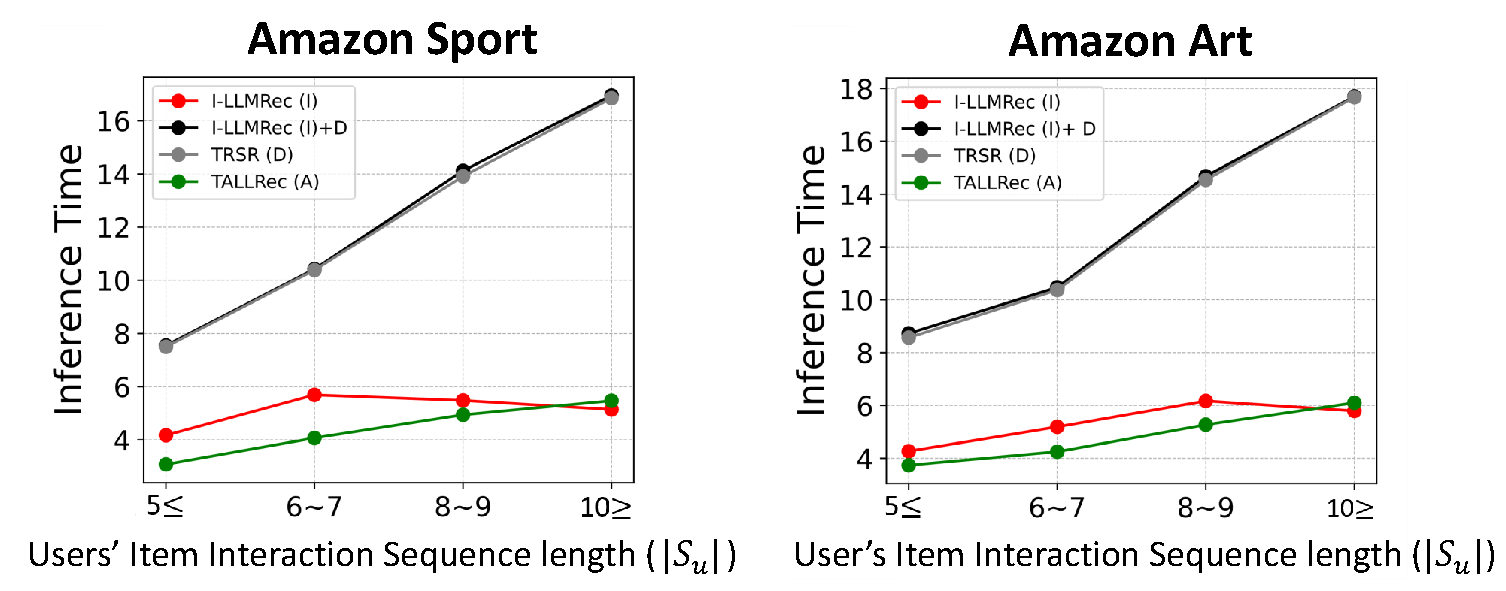
\includegraphics[width=.9\linewidth]{Figure/efficiency.pdf}
%         \vspace{-2ex}
%         \caption{Inference time (seconds/100 users) over the length of users' item interaction sequence (i.e., $|\mathcal{S}_u|$).}
%         \label{fig:efficiency}
%     \end{minipage}\hfill
%     % \vspace{-0.5ex}
%     \begin{minipage}{0.47\linewidth}
%         \centering
%         \vspace{-1.8ex}
%         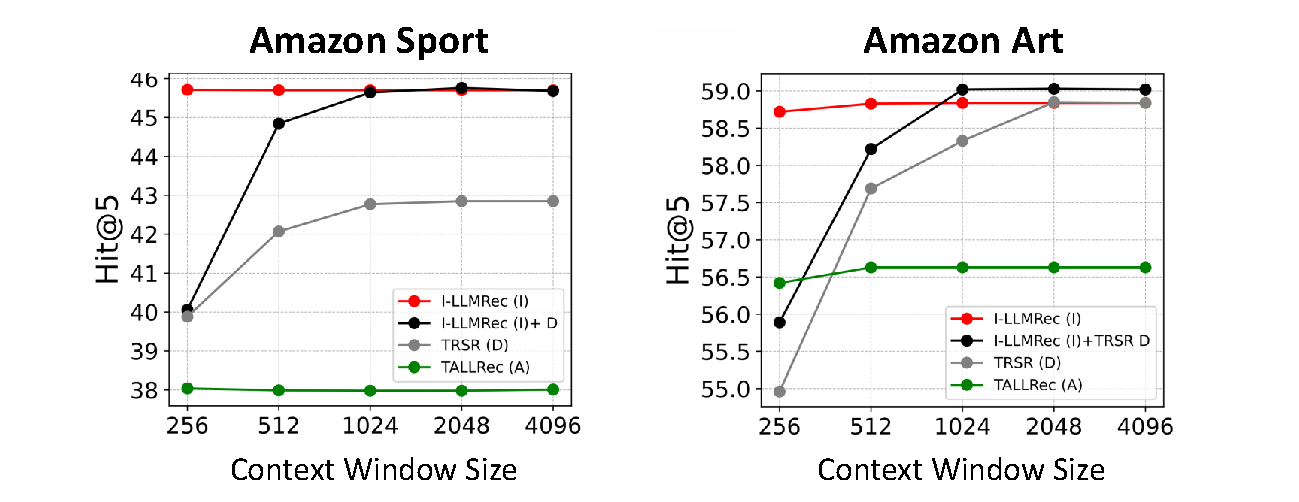
\includegraphics[width=.99\linewidth]{Figure/effectiveness.pdf}
%         \vspace{-3.3ex}
%         \caption{Performance of various LLM context window sizes.}
%     \label{fig:effectiveness}
%     \end{minipage}
%     \vspace{-2ex}
% \end{figure*}


\smallskip
\textbf{\textit{Image-aware LLM-based models}}.
\begin{itemize}[leftmargin=5mm]
    % \item \textbf{VIP5} \cite{geng2023vip5} express items using the image features and titles within the language model, recommending items based on their numerical IDs in natural language.
    \item \textbf{UniMP} \cite{wei2024towards} utilizes image features and attributes to represent items, and recommends them through image tokens assigned as out-of-vocabulary.
    \item \textbf{\proposed{}+$\mathbf{D}$ (equiv. to \proposed{}+TRSR)}\footnote{For each item in the user interaction, we append the description as "Description: $\mathbf{D}_i$" after $\mathbf{P}_i$ within the prompt, i.e., 
    $\mathbf{P}_i=\{ \textrm{Title}: \textsf{ITEM\_TITLE}, \textrm{Visual}\; \textrm{Representation}: [ \textsf{VISUAL}], \textrm{Description}: \textbf{D}_i$  \}} is a variant of \proposed{} that represent items using both image features and text description.
    % , combining the TRSR and \proposed{} approaches. 
\end{itemize}

% \textbf{LLM-based model}, and \textbf{Image-Aware LLM-based model}:

% 1) GRU4Rec \cite{hidasi2015session} employs the RNNs to capture sequential user interactions, VBPR \cite{he2016vbpr}  enhances BPR \cite{rendle2012bpr} by incorporating image features to improve personalized ranking, BERT4Rec \cite{sun2019bert4rec} applies bidirectional transformers with masked item prediction to capture complex user preference, SASRec \cite{kang2018self} uses self-attention mechanisms to capture long-term user preference. \textbf{2) LLM-based model}: TALLRec \cite{bao2023tallrec} converts numerical IDs into titles within the LLM. Beyond it, we add attributes (i.e., brand and category), to the title, regarding this model as a representative of the Attribute-based Representation approach, A-LLMRec \cite{kim2024large} combines the titles and CF item embeddings to express the items in order to recommend the warm items, and TRSR \cite{zheng2024harnessing} is a representative work of the Description-based Representation approach, which summarizes full item descriptions to effectively express items and leverage rich textual semantics. \textbf{3) Image-Aware LLM-based model}: VIP5 \cite{geng2023vip5} express items using the image features and titles within the language model, recommending items based on their numerical IDs in natural language, UniMP \cite{wei2024towards} utilizes image features and attributes to express the items and recommends them through image tokens allocated by out-of-vocabulary, Meanwhile, \proposed{}+$\mathbf{D}$\footnote{For each item in the user interaction, we append the description as "Description: $\mathbf{D}_i$" after $\mathbf{P}_i$ within the prompt.} is a variant of \proposed{} that express items using both image features and text description.


{Note that the main difference between LLM-based models and \proposed{} lies in how item semantics are represented (i.e., attributes, CF, descriptions, or images) in that both share the same LLM backbone and recommendation protocol.}

% \textbf{CF model}
% \begin{itemize}[leftmargin=5mm]
%     \item{GRU4Rec}
% \end{itemize}



\subsubsection{\textbf{Implementation Details}}
\label{sec:implementation}
We employed Sheared LLaMA 2.7B \cite{xia2023sheared} as the LLM backbone. For the visual encoder $V$, we adopt SigLIP \cite{zhai2023sigmoid}, a variant of CLIP \cite{radford2021learning} with a sigmoid loss function, to extract visual features. Regarding experiments with different LLMs and visual encoders, please refer to Appendix~\ref{app_sec:llm_visual}. We use a 2-layer MLP with ReLU activation function for the adaptor $M$. In IRE module, we employ SBERT \cite{reimers2019sentence} as the textual encoder. To ensure consistency across the LLM backbone, we use the same Sheared LLaMA 2.7B for TALLRec, A-LLMRec, and TRSR. Since these models are limited to recommending items only from a narrower item pool (i.e., 1 or 20), we apply the same IRE module for recommendation, which incorporates image, CF, and textual features, allowing them to recommend items from a larger pool. This approach is acceptable since our main goal is to evaluate how effectively the LLM captures user preferences through item expression. For TRSR, we use GPT-4o \cite{open2024gpt4o} to summarize full item descriptions. 
% Meanwhile, VIP5 follows its original implementation, using T5-Base \cite{raffel2020exploring} as its backbone, while
For UniMP, we follow its original implementation, which utilizes OpenFlamingo-4B-Instruct \cite{awadalla2023openflamingo}, a pre-trained multimodal LLM. Regarding training configurations, we set the learning rate to 0.001 and the batch size to 32. All models are trained on an NVIDIA GeForce A6000 48GB GPU.







% \vspace{-2ex}
\subsection{Performance Comparison (RQ1)}
\label{sec:performance}
Table~\ref{tab:main_table} shows the performance comparison between \proposed{} and baselines across four datasets. The key observations are as follows: \textbf{1)} LLM-based models generally outperform traditional CF models, highlighting the effectiveness of leveraging an LLM backbone for the recommender systems. 
\textbf{2)} A-LLMRec and TRSR generally outperform TALLRec. It suggests that beyond the attributes, incorporating CF item embeddings or item descriptions further enhances the LLM's ability to capture user preferences. However, we observe that A-LLMRec performs worse on the Phone dataset, and TRSR generally outperforms A-LLMRec, indicating that item descriptions are more effective than ID-based item embeddings in expressing item semantics.
\textbf{3)} \proposed{} outperforms UniMP, an image-aware LLM-based model. Given that UniMP employs a multimodal LLM where images and texts are pre-aligned, it indicates the need for a more specialized alignment strategy tailored to the recommendation tasks, demonstrating the effectiveness of \proposed{}.
% \textbf{4)} \proposed{} outperforms TRSR, implying that despite the information overlap between item image and description pairs as discussed in Section~\ref{sec:intro}, \textcolor{red}{text-specific information—expressed only through descriptions (e.g., material or purpose)—negatively impact recommendations, while most of the essential information for recommendation is already embedded within the overlapping information.
% }
\textbf{4)} {Considering that TRSR includes attributes during summarization (See Appendix~\ref{app_sec:prompt4summarization}), adding description information in TALLRec, which is equivalent to TRSR, improved performance, whereas descriptions in addition to images (i.e., \proposed{}+$\mathbf{D}$) did not improve the performance of \proposed{}.}
% descriptions in addition to images did not improve the performance of \proposed{} (\proposed{}+$\mathbf{D}$), while the performance is improved when adding descriptions to TALLRec (i.e., TRSR).
This suggests that while descriptions convey useful information, they are inherently limited by what is already present in images due to the significant information overlap between image and description pairs. Even if descriptions may include some text-specific information that images do not contain, the fact that performance remains competitive implies that such information has surprisingly little impact on the recommendations. This supports the idea that item images are sufficient to capture user preferences for recommendation.

% since image and description information heavily overlap, the information conveyed by descriptions is inherently limited by what is already present in images, supporting our observation in Section~\ref{sec:intro}. Even if descriptions may include some text-specific information that images do not contain, the fact that performance remains competitive implies that such information has little impact on the recommendations. This supports the idea that item images are sufficient to capture the user preferences.




\subsection{Model Analysis (RQ2)}
\label{sec:model_analysis}
In this section, we analyze how \proposed{}, which represents items using images, performs in recommendations compared to the natural language-based approach (TRSR, \proposed{}+$\mathbf{D}$, and TALLRec) in terms of efficiency, effectiveness, and robustness.




\begin{figure}[h]
        \centering
        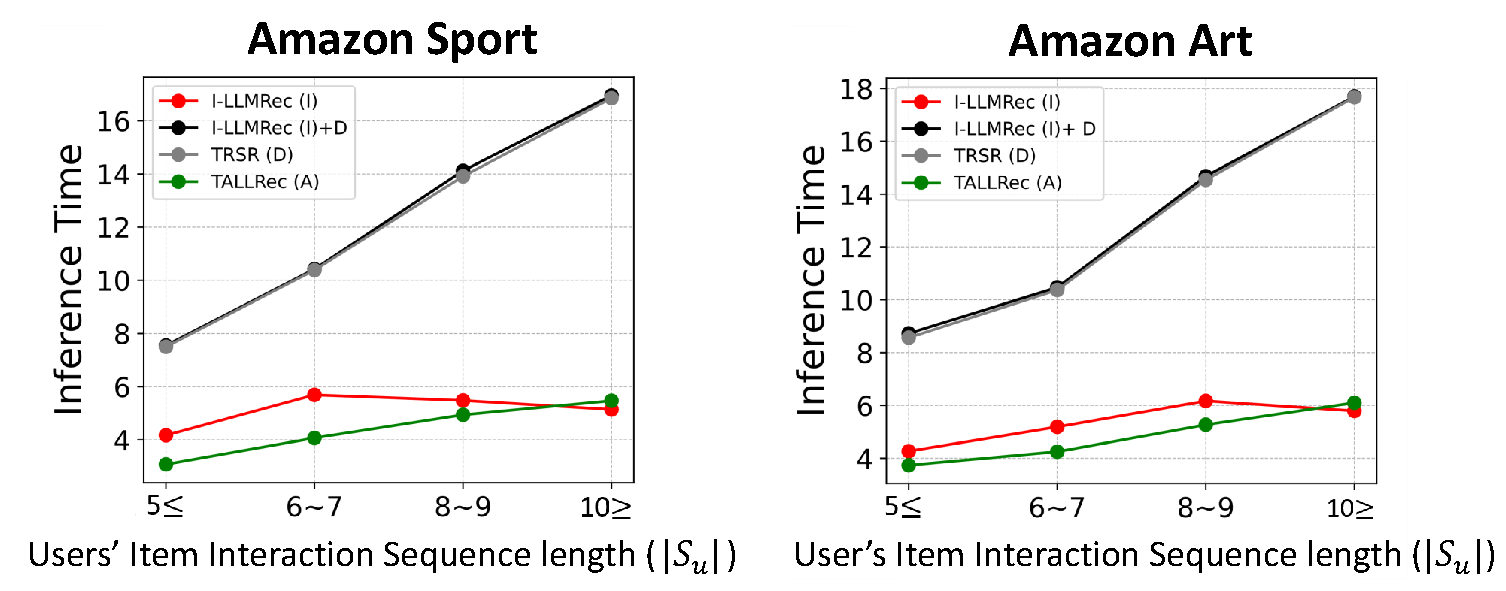
\includegraphics[width=.95\linewidth]{Figure/efficiency.pdf}
        \vspace{-1ex}
        \caption{Inference time (seconds/100 users) over the length of users' item interaction sequence (i.e., $|\mathcal{S}_u|$).}
        \label{fig:efficiency}
        \vspace{-1ex}
\end{figure}

\subsubsection{\textbf{Analysis on Efficiency.}} To study the efficiency of \proposed{}, we evaluate the inference time across different sizes of user's item interaction sequences (i.e., $|\mathcal{S}_u|$). Specifically, we divided the users into groups according to $|\mathcal{S}_u|$, randomly selected 100 users per group, and measured their total inference time. As shown in Figure~\ref{fig:efficiency}, we observe that TRSR and \proposed{}+$\mathbf{D}$, which rely on lengthy descriptions, show a sharp increase in inference time as the length of textual descriptions within the prompt increases proportional to $|\mathcal{S}_u|$. On the other hand, \proposed{} maintains consistently low inference time regardless of $|\mathcal{S}_u|$. This efficiency stems from the fact that even as $|\mathcal{S}_u|$ increases, only a minimal number of image tokens are added, keeping computational costs low. Furthermore, we observe that TALLRec, which is an attribute-based representation approach, shows a gradual increase in inference time and eventually surpasses \proposed{} when $|\mathcal{S}_u| \geq 10$. We attribute this to the fact that processing natural language attributes scales in complexity faster than image processing required for \proposed{}. In summary, \proposed{} is more efficient than TRSR across all $\mathcal{S}_u$ and even more efficient than TALLRec when user interactions are high, demonstrating superior computational efficiency.
\vspace{-1ex}

\begin{figure}[h]
        \centering
        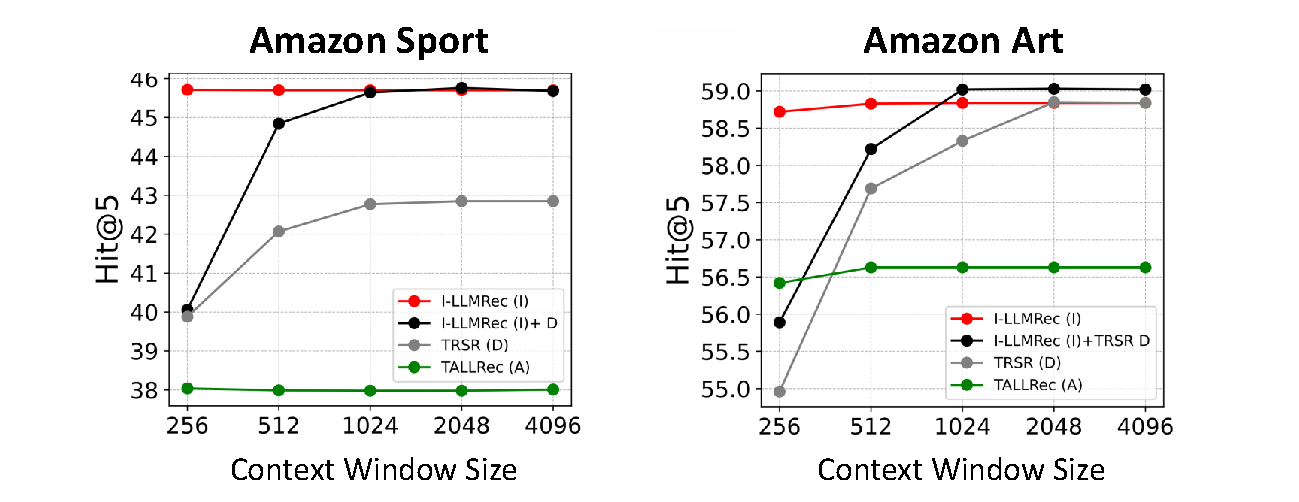
\includegraphics[width=.99\linewidth]{Figure/effectiveness.pdf}
        \vspace{-1ex}
        \caption{Performance of various LLM context window sizes.}
    \label{fig:effectiveness}
        \vspace{-1ex}
\end{figure}


% \vspace{-1.5ex}
\subsubsection{\textbf{Analysis on Effectiveness.}} 
To gain a deeper understanding of the effectiveness of \proposed{}, we examine how well it performs under a limited budget compared to the natural language-based approach. Specifically, we consider the LLM's context window size (i.e., maximum input token length) as the budget, and vary it from 4,096 to 256 tokens. This allows us to analyze the ability of models in effectively capturing the user preferences given a limited budget. As shown in Figure~\ref{fig:effectiveness}, we observe that TRSR, \proposed{}+$\mathbf{D}$, and \proposed{} perform consistently when the context window size is over 1,024 since they can handle most interactions. However, as the context window size drops below 512, the performance of TRSR and \proposed{}+TRSR declines sharply. This is because lengthy descriptions make it difficult for the LLM to fully process interactions with a limited context window size, thereby making it more challenging to understand user preferences. On the other hand, \proposed{} maintains stable performance even at the context window size of 256 by representing item semantics using minimal image tokens. This enables the LLM to process full user interactions within the given budget and effectively capture user preferences. While TALLRec also remains stable at 256 due to its low token usage, it exhibits inferior performance because its attributes are not expressive enough. Overall, \proposed{} effectively overcomes the context window size constraints by leveraging item images to preserve rich item semantics, demonstrating its effectiveness and practicality.





\begin{figure}[h]
        \centering
        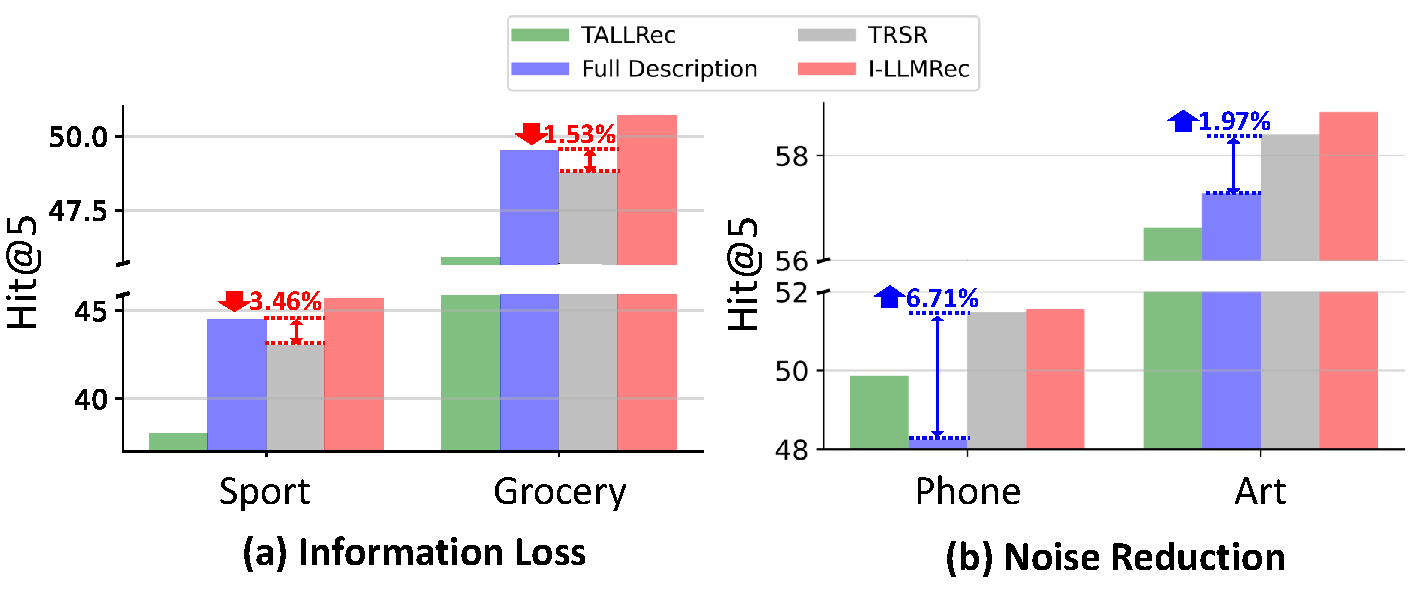
\includegraphics[width=.99\linewidth]{Figure/Robustness.pdf}
        \vspace{-1ex}
        \caption{Performance of natural language-based approaches  (TALLRec, TRSR and Full Description) and~\proposed{} on four datasets (Sports, Grocery, Phone and Art).}
        \label{fig:robust}
        \vspace{-1ex}
\end{figure}


\subsubsection{\textbf{Analysis on Robustness}}
\label{sec:robust}
To evaluate the robustness of representing items using images instead of natural language as done in \proposed{}, we compare its performance with various natural language-based approaches—TALLRec (Attribute), TRSR (Summarized description), and \textsf{Full description}—across multiple datasets. Figure~\ref{fig:robust} presents two key findings regarding the drawback of natural language-based approaches. \textbf{1) Information loss from summarization} (Figure~\ref{fig:robust}(a)): \textsf{Full description} outperforms TRSR, indicating that summarizing descriptions introduces information loss, where essential semantic details may be omitted, leading to lower performance. \textbf{2) Presence of Noise in Full Description} (Figure~\ref{fig:robust}(b)): On some datasets (i.e., Phone and Art), \textsf{Full description} rather performs worse than TRSR that relies on a summarized description. This indicates that the lengthy full description may contain noise and that the noise could be partially removed in the summarized version of the full description\footnote{Indeed, we found that full descriptions often contain extraneous content, such as HTML tags introduced during data crawling.}.
% This suggests that the negative impact of noise in full descriptions can sometimes outweigh the benefits of retaining complete information. 
Especially in Phone dataset, \textsf{Full Description} even underperforms TALLRec that relies only on simple attributes. 
Such different behaviors of natural language-based approaches across different datasets demonstrates that these approaches are sensitive to the given text, and thus impractical in reality.
% These findings highlight the sensitivity of natural language-based representation to both information loss and noise. 
In contrast, \proposed{}, which captures item semantics through images rather than text, consistently delivers strong performance across all datasets, 
% Unlike textual descriptions, images provide a more reliable and stable representation of item semantics. This consistent performance 
demonstrating its robustness in handling variations in item descriptions.

% evaluate sensitivity by comparing the performance of different natural language expression approaches, including the full description approach, and \proposed{} across diverse datasets. As shown in Figure~\ref{fig:robust},


% \noindent \textbf{Effectiveness over Limited Input Length.}

% \noindent \textbf{Efficiency over $|\mathcal{S}|_u$}



% \subsection{Discussion of Robustness}

% \vspace{-2ex}
\begin{table}[h]
\caption{Ablation studies of \proposed{}.}
\vspace{-1.0ex}
\resizebox{0.95\linewidth}{!}{
\begin{tabular}{c|c|ccc||cc|cc}
\toprule
\multirow{2}{*}{\textbf{Row}} & \multirow{2}{*}{\textbf{ILA}} & \multicolumn{3}{c||}{\textbf{IRE}} & \multicolumn{2}{c|}{\textbf{Sport}} & \multicolumn{2}{c}{\textbf{Art}}  \\ \cmidrule{3-9} 
                              &                                                                                      & Image           & CF             & Text           & \textbf{Hit@5}   & \textbf{NDCG@5}  & \textbf{Hit@5}  & \textbf{NDCG@5} \\ \midrule \midrule
(a)                           &                                                                                      & \ding{51}      &                &                &        0.3953          &        0.3043          & 0.5040          & 0.3915          \\
(b)                           & \ding{51}                                                                           & \ding{51}     &                &                & 0.4316           & 0.3403           & 0.5564          & 0.4447          \\
(c)                           & \ding{51}                                                                           &                 & \ding{51}     &                & 0.4075           & 0.3256           & 0.5502          & 0.4517          \\
(d)                           &\ding{51}                                                                          & \ding{51}     & \ding{51}     &                & 0.4491           & 0.3630           & 0.5795          & 0.4769          \\
(e)                           & \ding{51}                                                                          & \ding{51}      & \ding{51}     & \ding{51}     & \textbf{0.4570}  & \textbf{0.3711}  & \textbf{0.5883} & \textbf{0.4839} \\ \bottomrule
\end{tabular}
}
\label{tab:ablation}
\vspace{-1ex}
\end{table}

% \vspace{-2.0ex}
\begin{figure}[h]
        \centering
        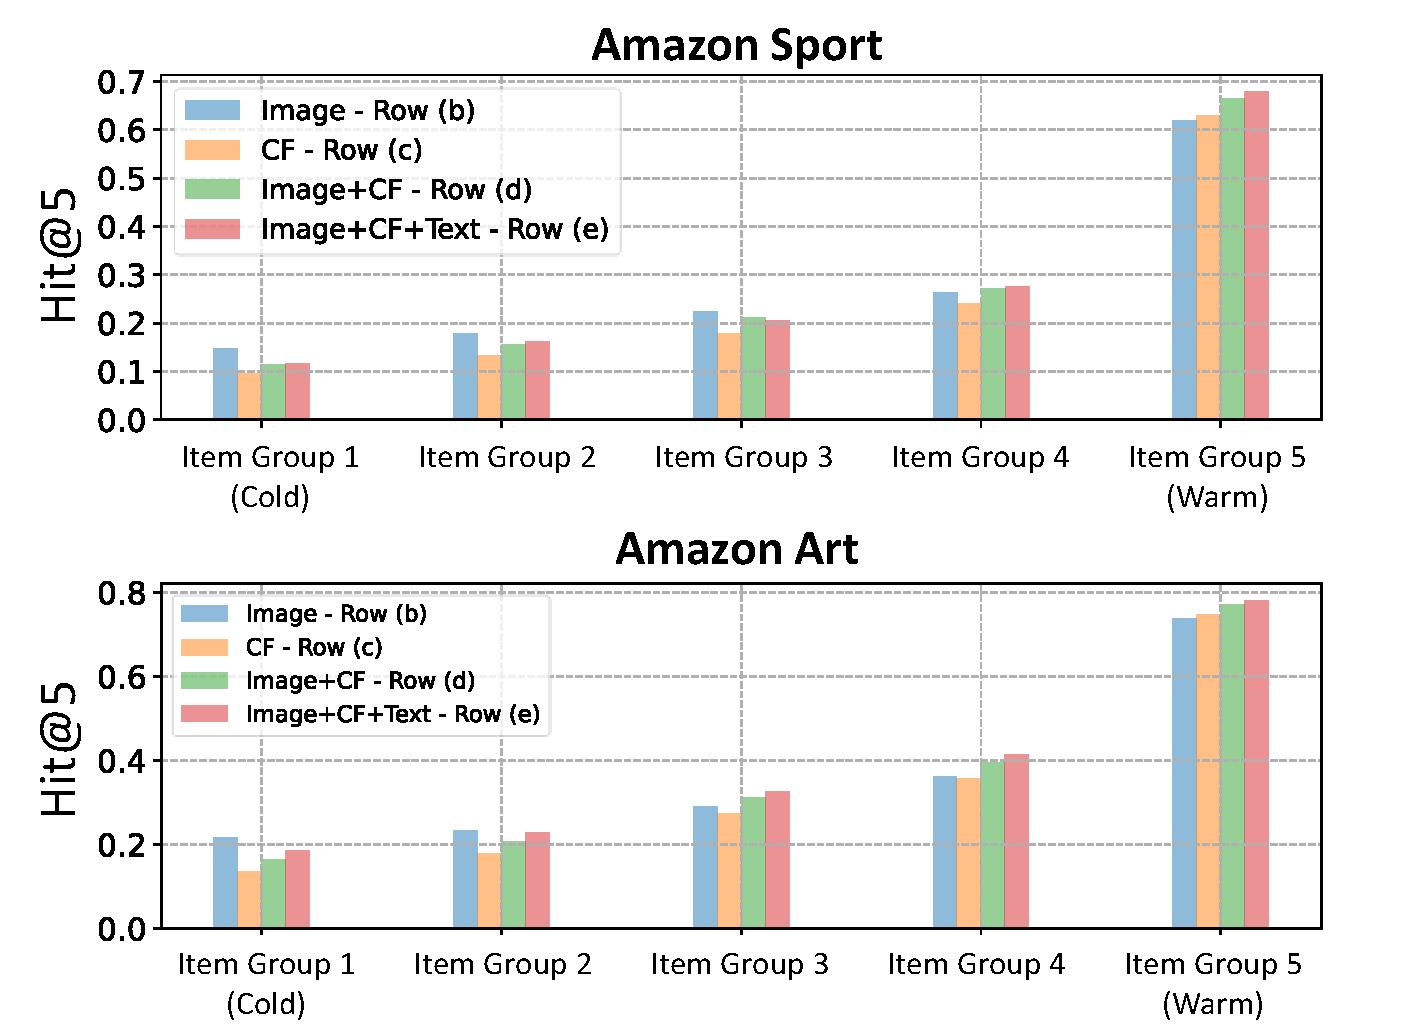
\includegraphics[width=.95\linewidth]{Figure/ablation_study.pdf}
        \vspace{-1ex}
        \caption{Performance across item groups, where higher IDs indicate warmer item groups.}
        \label{fig:ablation}
        \vspace{-1ex}
\end{figure}




\subsection{Ablation Studies (RQ3)}
\label{sec:ablation_study}
In Table~\ref{tab:ablation}, we conduct ablation studies to understand the effectiveness of each component in \proposed{}. The variant without any additional components is trained solely using Equation~\ref{eqn:5} and recommends items based only on image features (row (a)). We make the following observations: \textbf{1) Effect of ILA:} We observe that equipment with the ILA module significantly improves performance (row (a) vs. row (b)). This indicates that the ILA module effectively aligns visual features with the language space, enhancing the LLM's ability to understand user preferences. \textbf{2) Effect of extending to multiple feature types in IRE:} We observe that incorporating CF features along with image features\footnote{The inclusion of specific feature types is used for both the model training in Equation~\ref{eqn:7} and during inference in Equation~\ref{eqn:8}.} 
yields better performance than using either the image or CF feature alone (row (b), (c) vs. (d)). Moreover, integrating all three feature types (i.e., Image, CF, and Text) further improves performance (row (d) vs. (e)). This demonstrates that extending multiple feature types enhances recommendation effectiveness beyond image features alone.

\smallskip
\noindent \textbf{Effectiveness of Feature types across cold/warm items.} To further analyze the impact of different feature types, we evaluate their performance on cold and warm item recommendations. Specifically, we follow \cite{liu2023uncertainty} by sorting the items in ascending order based on the frequency of interaction and dividing them into five equally sized groups, where a higher group ID indicates a warmer item group, Then, we compare the recommendation performance across these groups. As shown in Figure~\ref{fig:ablation}, we observe that using image features (blue bar) generally outperforms CF features (orange bar) for cold items (lower ID groups). However, as the item group transitions from cold to warm, CF's effectiveness improves, eventually surpassing Image in Item Group 5 (Warm). This suggests that CF is particularly effective for recommending warm items. With these insights, combining Image and CF (green bar) helps mitigate CF's weakness in recommending cold items, resulting in higher performance than CF alone in Item Group 1-2. At the same time, the CF features compensate for weakness of the image features in recommending warm items, leading to better performance than image alone in Item Group 4-5. Furthermore, adding textual features (red bar) further boosts performance across all Item Groups, exceeding the performance of Image+CF. This analysis highlights how different feature types complement each other to enhance recommendation.




% \subsection{Missing Image Scenario (RQ4)}
% \label{exp:missing}
% In this section, we explore how to handle the miss




\begin{table}[h]
\caption{Performance when item images are missing.}
\vspace{-1.0ex}
\resizebox{0.95\linewidth}{!}{
\begin{tabular}{l|cc|cc}
\toprule
\multicolumn{1}{c|}{\multirow{2}{*}{}} & \multicolumn{2}{c|}{\textbf{Sport}} & \multicolumn{2}{c}{\textbf{Art}}  \\ \cmidrule{2-5} 
\multicolumn{1}{c|}{}                        & \textbf{Hit@5}   & \textbf{NDCG@5}  & \textbf{Hit@5}  & \textbf{NDCG@5} \\ \midrule \midrule
TALLRec                                      & 0.3801           & 0.2938           & 0.5663          & 0.4572          \\
TRSR                                         & 0.4302           & 0.3375           & \textbf{0.5841} & 0.4758          \\
\proposed{} w/ missing images             & \textbf{0.4451}  & \textbf{0.3589}  & 0.5805          & \textbf{0.4789} \\ \bottomrule
\end{tabular}
}
\vspace{-1ex}
\label{fig:missing}
\end{table}

\subsection{Missing Image Scenario (RQ4)}
\label{app_sec:missing_image}
In this section, we explore how to handle scenarios where item images are missing and evaluate how effectively we can manage them. Specifically, we randomly remove 50\% of the item images from the entire item pool. As a result, these missing images cannot be used for item semantics representation (Equation~\ref{eqn:2}) and retrieval-based recommendation (Equation~\ref{eqn:5} and Equation~\ref{eqn:8}). To compensate for the missing images, we substitute them with readily available textual descriptions. 
% More precisely, instead of using images, we represent the semantics of these items using text descriptions to capture user preferences. 
Similarly, for retrieval-based recommendations, when item images are missing, we extract textual features derived from descriptions using SigLIP \cite{zhai2023sigmoid} text encoder rather than extracting visual features from images using SigLIP visual encoder. 
% Since SigLIP jointly embeds image and language representations, this ensures a seamless replacement without introducing a representation gap. 
As shown in Table~\ref{fig:missing}, \proposed{} trained with half of the items missing images outperforms the baselines (TALLRec and TRSR), even though the baselines were trained without any missing item images. This demonstrate the effectiveness of~\proposed{} in handling the missing image scenario, which shows the practicality of~\proposed{} in reality.
% . Considering that TALLRec and TRSR utilize the complete set of item images for recommendations, while \proposed{} uses only half of the item images, it is reasonable that \proposed{} shows a slight performance decline compared to TRSR on the Art dataset.


\section{Related Work}
\noindent\textbf{Sequential Recommendation. }
Our setup closely aligns with the sequential recommendation, where a user's item interaction history is listed as a sequence in chronological order, and the goal is to predict the user's next interaction item. Early studies process user sequences via the Markov chain for sequential recommendation \cite{he2016fusing,mahmood2007learning,wang2015learning}. With the advancement of deep learning, RNNs were used for sequence modeling to capture user preference \cite{hidasi2015session,li2017neural}, while studies using CNN treat previous interacted items' embedding matrices as images, enabling the convolutional operation to consider user sequences \cite{tang2018personalized,yuan2019simple,kim2016convolutional}.
Recently, with the emergence of Transformer \cite{vaswani2017attention}, the self-attention mechanism has been applied to sequential recommendations \cite{kang2018self,sun2019bert4rec,xu2021long}. More recently, the focus has shifted towards leveraging rich side information associated with items (e.g., images or text) in the sequential recommendation. Specifically, TempRec \cite{wu2022news} encodes textual information of items to strengthen item embeddings, while MMMLP \cite{liang2023mmmlp} fuses visual and textual features in the user sequence to capture fine-grained user preferences. 

% \textcolor{blue}{hong: below paragraph I think, maybe more fits as the starter of LLM-based Recommendation. Too many transitions in here. Sequential=>Multi-modal sequential => LLM rec}
% However, they overlook the strong generalization capabilities of LLMs, which limits the exploration of their potential advantages in areas such as few-shot/zero-shot recommendations \cite{bao2023tallrec,wang2023zero}, cross-domain recommendations \cite{kim2024large}, cold-start user/item recommendations \cite{zhang2023collm,liu2024once} and etc.



\smallskip
\noindent\textbf{LLM-based Recommendation. }
Due to the power of textual understanding and world knowledge of LLMs, a myriad of studies have spurred the development of LLMs for recommender systems \cite{bao2023tallrec, wang2023zero,kim2024large,zhang2023collm, liu2024once}. 
% Specifically, they are known to be effective in addressing the limitations of traditional recommender systems such as few-shot/zero-shot recommendations, and cold-start user/item recommendations \cite{bao2023tallrec, wang2023zero,kim2024large,zhang2023collm, liu2024once}.
% Most of the LLM-based recommender systems transform the numerical ID of items to natural language forms (e.g., item titles) to fully leverage the LLMs' comprehensive understanding of natural language \cite{bao2023tallrec, kim2024large, zhang2023collm, LLaRA2024}.
% To fully leverage the LLMs' comprehensive understanding of natural language, most of the LLM-based recommender systems transform the traditional numerical ID to natural language forms (e.g., item title).
% , thereby capturing the user preferences based on the semantic understanding of user sequence. 
To adapt LLMs for recommendation tasks, previous studies represent the interaction history as a sequence of item titles.
Additionally, some studies enhance recommendation performance by incorporating item attributes, providing richer item semantics to the LLMs (\textbf{Attribute-based Representation}).
% Previous studies represent the user's interaction history as a sequence of item titles combined with simple attributes (i.e., category, brand, etc.) \textbf{Attribute-based Representation}.
Specifically, TALLRec \cite{bao2023tallrec} converts item IDs into their titles and captures user preference via LoRA \cite{hu2021lora} fine-tuning. TransRec \cite{lin2024bridging} improves the user preference understanding by including item titles and attributes in prompts. IDGenRec \cite{tan2024idgenrec} incorporates item titles generated by an independent LLM for unique and meaningful semantics.
% More recently, TRSR \cite{zheng2024harnessing} utilizes a large LLM (i.e., LLaMA-30B-instruct \cite{touvron2023llama}) to summarize item descriptions, and feeds the condensed and meaningful information to the smaller LLMs for recommendation.
More recently, to feed the richer item semantics to LLMs, a description of items have been utilized (\textbf{Description-based Representation}).
% More recently, the items' richer textual semantics (i.e., description) have been leveraged to represent items (\textbf{Description-based Representation}).
Specifically, TRSR \cite{zheng2024harnessing} utilizes a large LLM (i.e., LLaMA-30B-instruct \cite{touvron2023llama}) to summarize item descriptions, and feeds them to a smaller LLM (i.e., LLaMA-2 7B \cite{touvron2023llama2}) to capture the condensed meaningful information, while ONCE \cite{liu2024once} adopts GPT-3.5 \cite{brown2020language} for the summarizing task.
% ONCE \cite{liu2024once} represents items by summarizing their textual content using GPT-3.5 \cite{brown2020language}, following by inserting them into the prompts of a smaller LLM (i.e., LLaMA-7B).
Despite their notable success to capture the richer item semantics, they face a trade-off between efficiency and effectiveness when representing items in natural language, leading us to utilize image information to address this trade-off.
Meanwhile, VIP5 \cite{geng2023vip5} and UniMP \cite{wei2024towards} have attempted to incorporate image information into LLMs. However, they lack an in-depth investigation into the overlap between image-description pairs and fail to provide effective alignment strategies between image and language spaces tailored to the recommendation context.

% \subsection{Aligning Modality with LLMs}
% \textcolor{blue}{With the rapid advancement of LLMs, researchers have explored integrating various modalities (e.g., image and video) with LLMs to perform multimodal tasks beyond natural language tasks. However, since LLMs are primarily trained for language modeling, understanding modalities such as images or videos is unfeasible. To address this limitation, several studies have explored on introducing modalities into LLMs \cite{liu2024visual,li2023blip,li2023videochat,lin2024vila,tang2024graphgpt}. One promising approach involves aligning modality embeddings with the LLM's language space, enabling LLMs to understand the information of modality in the embedding space \cite{li2023blip, liu2024visual, yin2024lamm}. Specifically, BLIP2 \cite{li2023blip} employs a Transformer-based adaptor to align image embeddings with LLMs, while LLaVA \cite{liu2024visual} uses visual instruction tuning. Furthermore, LAMM \cite{yin2024lamm} aligns 3D modality using 3D point cloud instruction tuning. Inspired by these effective alignment strategies for multimodalities, we propose a novel approach for aligning images with LLMs within the recommendation system. Instead of representing items with textual descriptions, we align images with LLMs to address the trade-off problem more efficiently.}

% With the rapid advancement of LLMs, researchers have explored integrating diverse modalities (e.g., images, videos) with LLMs beyond natural language to perform multimodal-language tasks.
% Specifically, LLaVA \cite{liu2024visual} aligns image and language spaces in LLMs through visual instruction tuning, enabling vision-language tasks. VideoChat \cite{li2023videochat} constructs a video instruction tuning dataset and performs instruction tuning to align video space with LLMs, facilitating video-language tasks. Similarly, LAMM \cite{yin2024lamm} aligns the 3D modality through 3D point cloud instruction tuning, enabling 3D grounding tasks. 
% Inspired by these studies on multimodal alignment with LLMs, we propose aligning images with LLMs in the context of recommendation systems. Instead of representing items with descriptions, we align images with LLMs to address the trade-off problem effectively.

\vspace{-1ex}
\section{Conclusion}
\label{sec:conclusion}
In this work, we address the trade-off between efficiency and effectiveness when representing item semantics in natural language for an LLM-based recommender system. Based on the observation that there exists a significant information overlap between images and descriptions associated with items, we propose \proposed{}, a novel method that leverages images to capture rich item semantics of lengthy descriptions with only a few tokens, thereby capturing user preferences efficiently and effectively. However, as the image and language space are not inherently aligned, we propose the Image-LLM Alignment (ILA) mode, which effectively bridges the gap between these spaces. Furthermore, we propose the Image-based REtrieval (IRE) mode, a retrieval-based recommendation approach, to enhance both the reliability and efficiency of the recommender systems. Our extensive experiments demonstrate that \proposed{} outperforms natural language-based approaches in terms of both efficiency and effectiveness.

\normalem
\bibliographystyle{ACM-Reference-Format}
\bibliography{MLLMRec}


\appendix

% \newpage

\clearpage

\section{Ethics Statement}
To the best of our knowledge, we comply with the KDD Code of Ethics and do not violate any ethical issues. Throughout this paper, we use publicly available data and code.

\begin{figure}[h]
        \centering
        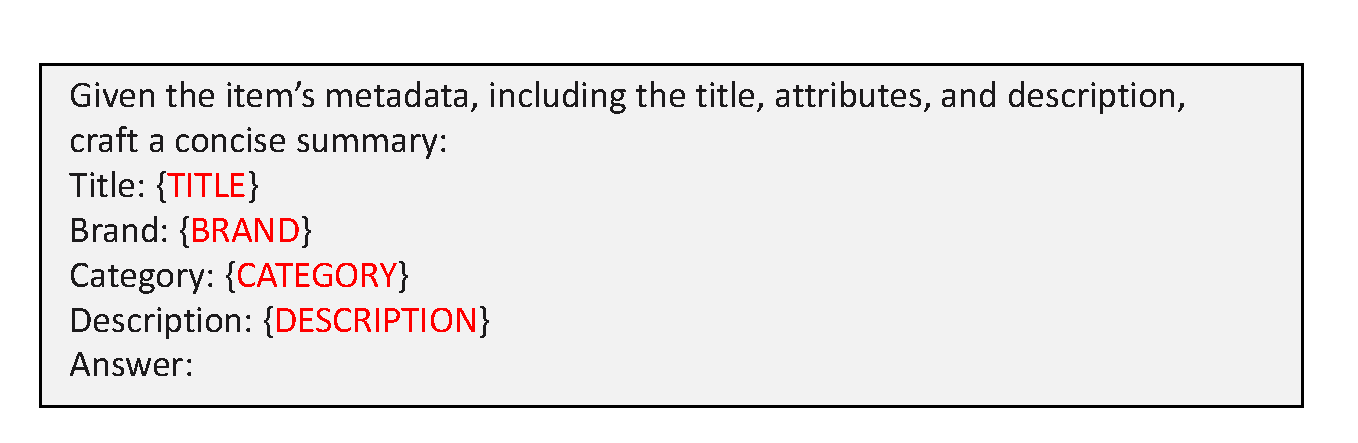
\includegraphics[width=.90\linewidth]{Figure/Prompt_summarization.pdf}
        \vspace{-2ex}
        \caption{Prompt for summarizing descriptions. The red-colored text denotes the actual metadata for the item.}
        \label{fig:prompt_summarization}
        \vspace{-2ex}
\end{figure}

\section{Prompt for Summarization}
\label{app_sec:prompt4summarization}
Figure~\ref{fig:prompt_summarization} shows the prompt used for description summarization. Following TRSR \cite{zheng2024harnessing}, we incorporate attribute information along with the description to generate a concise summary. 


\section{Recommendation Protocol}
\label{app_sec:rec_protocol}
In this section, we describe a comprehensive explanation of the recommendation protocol, which is consistently applied to Attribute-based Representation, Description-based Representation (i.e., Full Description and Summarized Description), and \proposed{} as introduced in Section~\ref{sec:intro}. Note that this recommendation protocol follows a retrieval-based recommendation approach similar to the IRE module discussed in Section~\ref{sec:retrieval}. Therefore, we recommend reading Section~\ref{sec:retrieval} first for a deeper understanding.
At a high level, we modify the way items are represented by replacing the visual representation with either an attribute-based or description-based representation within Equation~\ref{eqn:2}, followed by a recommending process similar to IRE module.
% we just replace the visual representation in Equation~\ref{eqn:2} with the attributes or the descriptions depending on the

Specifically, we first craft the prompt, which includes the task prompt (as shown in Figure~\ref{fig:main}) and the semantics of user-interacted items in a sequence. Here, the item semantics depend on the item representation approach, which plays a crucial role in capturing user preferences. Then, we append a learnable token \rectoken{} at the end, allowing this token to aggregate the semantics of items the user has interacted with, thereby capturing user preferences. To obtain the corresponding representation, we use the last hidden state of \rectoken{} token, which serves as the LLM-guided user representation. Using this representation, we retrieve relevant items by comparing with items' visual, collaborative filtering (CF), and textual features.
More precisely, for each feature type, we compute affinity scores by performing a dot-product between the LLM-guided user representation and item features. Based on the summation of affinity score across feature types for all items, we rank the items and recommend the Top-$k$ items with the highest scores. 




\begin{figure}[h]
  \centering
  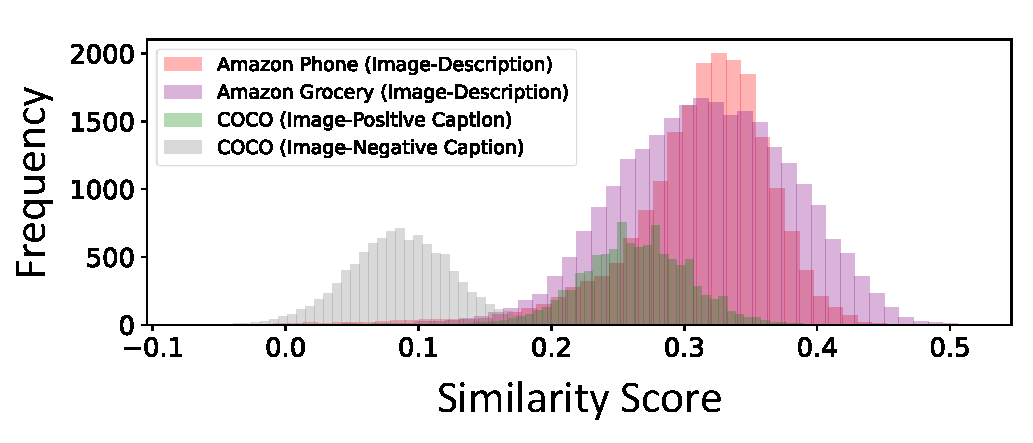
\includegraphics[width=0.95\linewidth]{Figure/Appendix_overlap.pdf}
  \vspace{-3.5ex}
  \caption{Cosine similarity between item image-description pairs in Amazon Phone and Grocery datasets and image-caption pairs in the COCO dataset using CLIP \cite{radford2021learning}.}
  \label{app_fig:cosine}
  \vspace{-1ex}
\end{figure}


\begin{figure}[h]
  \centering
  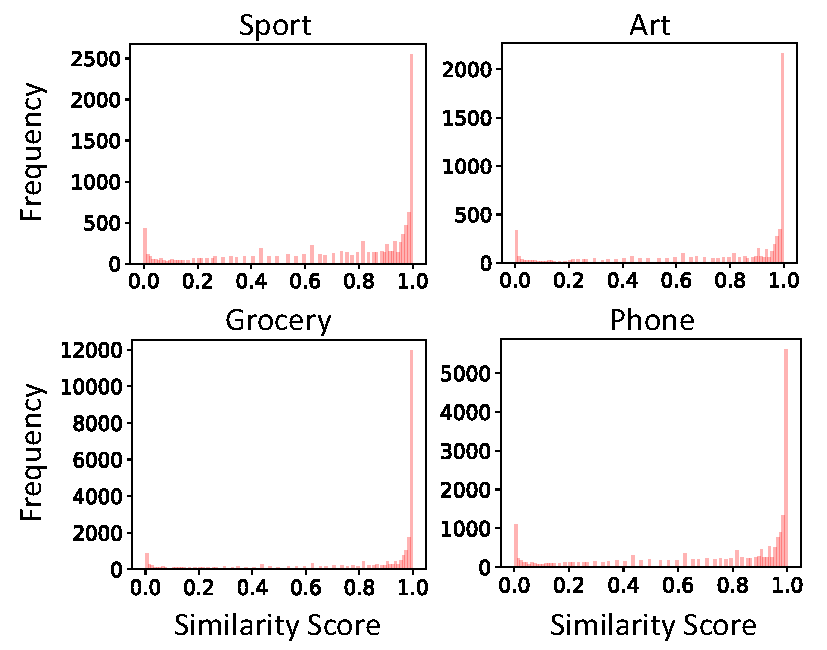
\includegraphics[width=0.95\linewidth]{Figure/Siglip_overlap.pdf}
  % \vspace{-3.5ex}
  \caption{Sigmoid-based similarity (ranging from 0 to 1) between item image-description pairs across four datasets (Amazon Sport, Art, Grocery, and Phone datasets) using SigLIP \cite{zhai2023sigmoid}.}
  \label{app_fig:siglip}
  \vspace{-2ex}
\end{figure}



\section{Consistent Observation of Information Overlap}
\label{app_sec:overlap_other_dataset}
We further investigate the information overlap between image and description associated with items, which was explored in Section~\ref{sec:intro}, by expanding these experiments to additional datasets and leveraging another CLIP=based model. \textbf{1) Expanding to additional datasets:} Building upon our previous comparative experiments in Amazon Sport and Art—where we used CLIP \cite{radford2021learning} to measure cosine similarity in Section~\ref{sec:intro}—we extend our analysis to the Amazon Grocery and Phone datasets. As shown in Figure~\ref{app_fig:cosine}, the average similarity for Amazon Phone and Grocery is approximately 0.31, which is higher than 0.26 average similarity observed in well-aligned COCO image-caption pairs. This consistent observation across multiple datasets further supports the information overlap between item images and descriptions. \textbf{2) Leveraging another CLIP model:} To further explore the information overlap using a different CLIP variant, we select SigLIP \cite{zhai2023sigmoid}, a variant of CLIP with sigmoid loss function, to compute the similarity scores ranging from 0 to 1. Specifically, when we apply SigLIP to measure similarity between item image-description pairs across all four datasets (Amazon Sport, Art, Grocery, and Phone), we observed that, as show in Figure~\ref{app_fig:siglip}, the majority of items exhibit similarity scores close to 1, further demonstrating the significant information overlap between their image and description pairs.

% conducted additional experiments using different CLIP model, SigLIP \cite{zhai2023sigmoid}, a variant of CLIP with sigmoid loss function, to measure the similarity ranging from 0 to 1. Specifically, this model allows us to measure the 













\begin{table}[h]
\caption{Performance comparison when LLM backbone of ~\proposed{} is fine-tuned using LoRA \cite{hu2021lora}.}
\vspace{-2.0ex}
\resizebox{.9\linewidth}{!}{
\begin{tabular}{l|cc|cc}
\toprule
\multirow{2}{*}{} & \multicolumn{2}{c|}{\textbf{Sport}} & \multicolumn{2}{c}{\textbf{Art}} \\ \cmidrule{2-5} 
                  & \textbf{Hit@5}   & \textbf{NDCG@5}  & \textbf{Hit@5} & \textbf{NDCG@5} \\ \midrule \midrule
LLM Frozen        & 0.4570           & 0.3711           & 0.5883         & 0.4839          \\
LLM fine-tuning with LoRA       &    \textbf{0.4633}              &   \textbf{0.3772}               &     \textbf{0.5958}           & \textbf{0.4949}                 \\ \bottomrule
\end{tabular}
}
\label{app_tab:lora}
\end{table}


\section{Frozen LLM vs LoRA Fine-Tuned LLM}
\label{app_sec:fine_tune}
Note that fine-tuning the LLM backbone is not mandatory for~\proposed{}. Nevertheless, in this section, we explore potential performance gains from fine-tuning the LLM, a common approach in existing LLM-based recommender systems \cite{lin2024bridging,bao2023tallrec,tan2024idgenrec,zheng2024harnessing,liu2024once}. However, since fully fine-tuning an LLM demands substantial computational resources, we adopt the parameter-efficient fine-tuning strategy, LoRA \cite{hu2021lora}, which introduces a small number of learnable rank matrices into each LLM's transformer layer. As shown in Table~\ref{app_tab:lora}, we observed the performance improvement through fine-tuning, indicating that there is room for further improvement within \proposed{}. However, considering the computational cost, we opt to freeze the LLM to preserve its intrinsic knowledge while improving training efficiency.



\begin{table}[h]
\caption{Data statistics after preprocessing.}
\vspace{-2.5ex}
\resizebox{0.95\linewidth}{!}{
\begin{tabular}{c|cccc}
\toprule
\textbf{Dataset} & \textbf{\# Users} & \textbf{\# Items} & \textbf{\# Interactions} & \textbf{Avg. Len} \\ \midrule \midrule
Sport            & 24,665            & 9,884             & 179,491                  & 7.28              \\
Grocery          & 84,896            & 25,632            & 739,628                  & 8.71              \\
Art              & 14,986            & 5,801             & 121,917                  & 8.13              \\
Phone            & 59,307            & 19,671            & 403,194                  & 6.80              \\ \bottomrule
\end{tabular}
}
\label{tab:statistics}
\vspace{-2ex}
\end{table}



\section{Data Statistics}
\label{app_sec:data_statistics}
Table~\ref{tab:statistics} shows the summary of the data statistics after preprocessing. Our experiments were conducted on datasets of varying scale, ranging from Grocery, which has a large number of interactions, to Art, which has relatively fewer interactions.



\begin{table}[h]
\caption{Impact of the different backbones.}
\vspace{-2.0ex}
\resizebox{.95\linewidth}{!}{
\begin{tabular}{c|c|cc|cc}
\toprule
\multirow{2}{*}{\textbf{LLM}} & \multirow{2}{*}{\textbf{Vision Encoder}} & \multicolumn{2}{c|}{\textbf{Sport}} & \multicolumn{2}{c}{\textbf{Art}} \\ \cmidrule{3-6} 
                     &                                 & \textbf{Hit@5}        & \textbf{NDCG@5}      & \textbf{Hit@5}      & \textbf{NDCG@5}     \\ \midrule \midrule
LLaMA-2.7B         & SigLIP                      & \textbf{0.4570}       & \textbf{0.3711}      & \textbf{0.5883}     & \textbf{0.4839}     \\
LLaMA-2.7B         & CLIP                        & 0.4476       & 0.3560      & 0.5836     & 0.4796     \\ \midrule
Vicuna 1.5-7B           & SigLIP                      &        \textbf{0.4670}      & \textbf{0.3779}            &    \textbf{0.5943}        &  \textbf{0.4930}         \\
Vicuna 1.5-7B           & CLIP                        &     0.4552         &     0.3677        &     0.5885      &   0.4892         \\ \bottomrule
\end{tabular}
}
\label{app_tab:diverse}
\end{table}

\section{Impact of Different LLMs and Vision Encoders}
\label{app_sec:llm_visual}
To investigate the impact of the backbone models on the recommendation performance of ~\proposed{}, we evaluated our model by replacing different backbone models.
For the LLM, we used Sheared LLaMA-2.7B \cite{xia2023sheared} and Vicuna 1.5-7B \cite{chiang2023vicuna}, an improved version of LLaMA-7B \cite{touvron2023llama}. For the vision encoder, we used CLIP\footnote{https://huggingface.co/openai/clip-vit-large-patch14-336} \cite{radford2021learning} and SigLIP\footnote{\url{https://huggingface.co/google/siglip-so400m-patch14-384}} \cite{zhai2023sigmoid}, with the advanced version of CLIP scaling with sigmoid loss.
Table \ref{app_tab:diverse} shows the following observations: 1) Given the same vision encoder, \proposed{} with Vicuna 1.5-7B outperforms the model with LLaMA-2.7B. This improvement is likely attributed to Vicuna 1.5-7B's superior semantic reasoning capability, allowing it to capture user preferences more effectively. 
2) Given the same LLM backbone, \proposed{} with SigLIP performs better than the version with CLIP. This suggests that models that better capture visual features are more effective in delivering item semantics, thereby enabling the LLM to better understand the item semantics.
In summary, employing more powerful LLMs and vision encoders leads to improvements in recommendation performance, as these models effectively capture item semantics and user preference.






\section{Training Strategy}
\label{app_sec:train_strategy}
Throughout this paper, we optimize our model using an end-to-end training strategy to ensure ease of implementation and learning efficiency. However, in this section, we explore the impact of an alternative two-stage training strategy, where we separate the ILA and IRE modules. Specifically, for stage 1, we train the adaptor $M$ through the ILA module to initially align the visual space with the language space. For stage 2, we freeze the adaptor and train only $F_u^*$ and $F_i^*$ ($*$=[\textsf{Img}, \textsf{CF}, \textsf{Text}]) through the IRE module. As shown in Table~\ref{app_tab:train_strategy}, the two-stage strategy shows performance comparable to the end-to-end strategy, indicating that neither strategy offers a clear advantage over the other. Given this, we opt for the end-to-end training strategy to facilitate the ease of implementation and training efficiency.







\begin{table}[h]
\caption{Training Strategy.}
\vspace{-2ex}
\resizebox{0.95\linewidth}{!}{
\begin{tabular}{l|cc|cc}
\toprule
\multirow{2}{*}{\textbf{Training Strategy}} & \multicolumn{2}{c|}{\textbf{Sport}} & \multicolumn{2}{c}{\textbf{Art}} \\ \cmidrule{2-5} 
                  & \textbf{Hit@5}   & \textbf{NDCG@5}  & \textbf{Hit@5} & \textbf{NDCG@5} \\ \midrule \midrule
End-to-End        & 0.4570           & 0.3711           & 0.5883         & 0.4839          \\
Stage1+Stage2     &       0.4604           &  0.3747                 &      0.5858          &    0.4887             \\ \bottomrule
\end{tabular}
}
\label{app_tab:train_strategy}
\end{table}





% \section{Qualitative Result of efficient alignment}
% \label{app_sec:qualitative}
% To demonstrate the effectiveness of alignment between visual and language space via the ILA module, we 


\begin{figure*}[t]
        \centering
        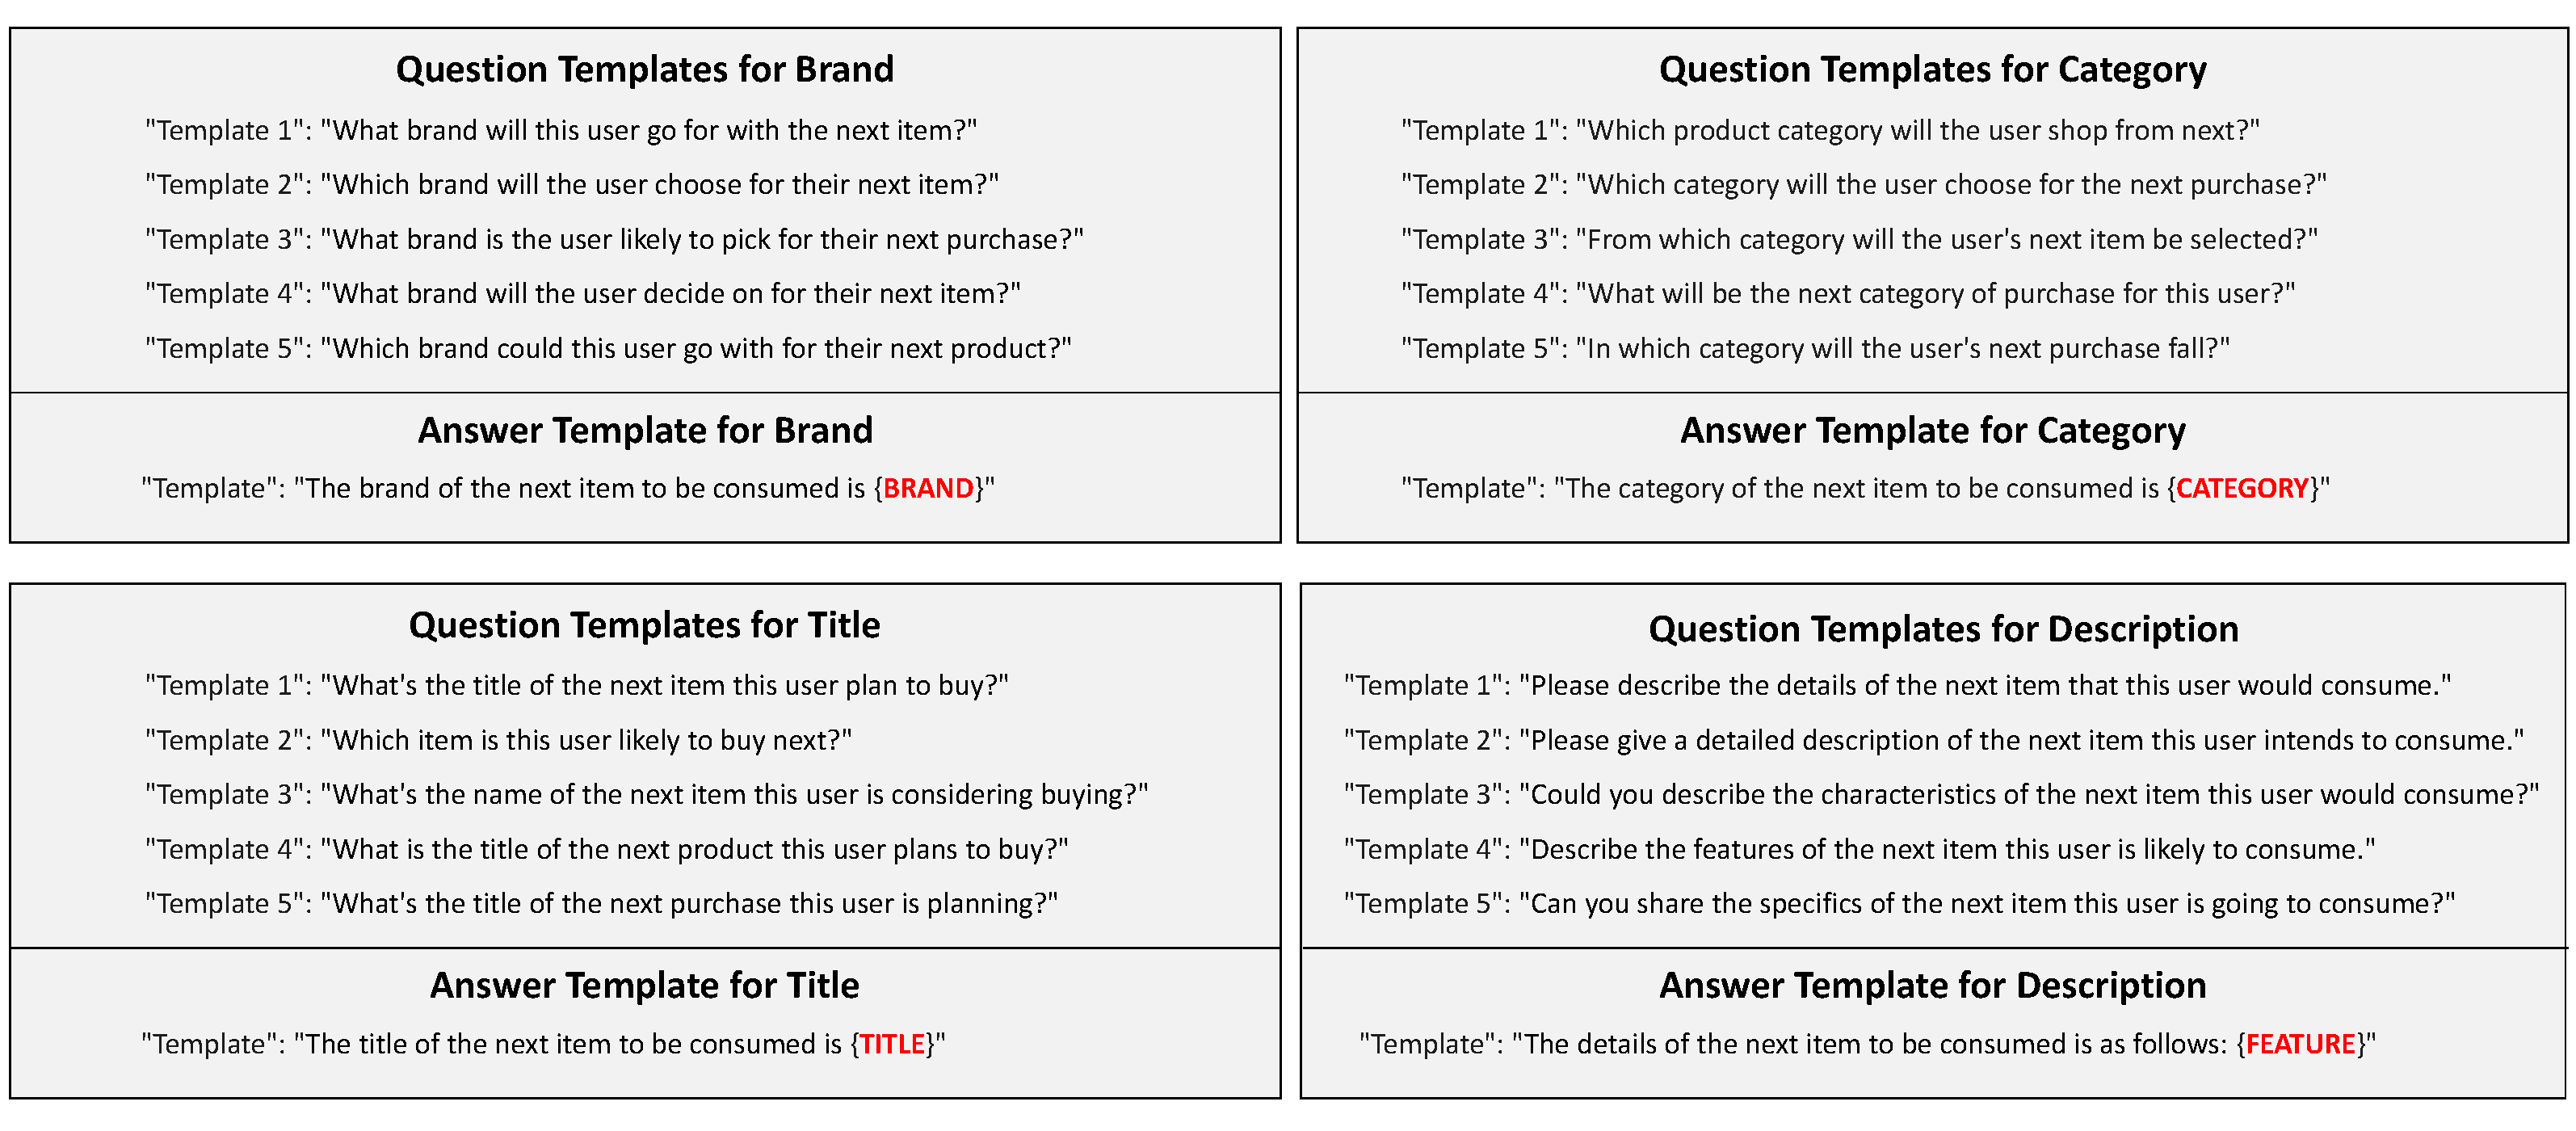
\includegraphics[width=.99\linewidth]{Figure/template.pdf}
        \vspace{-2ex}
        \caption{Prompt template for ILA module. The red-colored text denotes the actual information of an item.}
        \vspace{-0.5ex}
        \label{fig:template}
\end{figure*}

\section{ILA Prompt Templates}
\label{app_sec:question}
Figure \ref{fig:template} shows the prompt template for ILA module of ~\proposed{}. As described in Section \ref{sec:alignment}, we utilize the prompt templates to align the visual feature with the language space of LLMs by training the adaptor network $M$.

\end{document}
% \endinput
%%
%% End of file `sample-sigconf.tex'.
